% =====================================================================
% UniBus Live — B.Sc. Thesis Book
% Department of Computer Science and Engineering
% NPI University of Bangladesh
% Compile: pdflatex main.tex  (run twice for TOC/refs)
% =====================================================================
\documentclass[12pt, a4paper, oneside]{report}

% ---------- typography & layout ----------
\usepackage[T1]{fontenc}
\usepackage[utf8]{inputenc}
\usepackage{mathptmx}                     % Times-like text and math
\usepackage[a4paper, left=1.5in, right=1in, top=1in, bottom=1in]{geometry}
\usepackage{setspace}
\onehalfspacing
\usepackage{parskip}
\setlength{\parindent}{0pt}

% ---------- packages ----------
\usepackage{graphicx}
\usepackage{xcolor}
\usepackage{booktabs}
\usepackage{array}
\usepackage{longtable}
\usepackage{url}
\usepackage{float}
\usepackage{amsmath,amssymb}
\usepackage{algorithm}
\usepackage{algpseudocode}
\usepackage{caption}
\captionsetup{font=small, labelfont=bf}
\usepackage{tikz}
\usetikzlibrary{positioning, arrows.meta, calc}
\usepackage{enumitem}
\setlist{topsep=2pt, itemsep=2pt, parsep=0pt}
\usepackage[hidelinks]{hyperref}

% ---------- headers ----------
\usepackage{fancyhdr}
\setlength{\headheight}{15pt}
\pagestyle{fancy}
\fancyhf{}
\fancyhead[L]{\small\nouppercase{\leftmark}}
\fancyhead[R]{\small\thepage}
\renewcommand{\headrulewidth}{0.3pt}
\fancypagestyle{plain}{\fancyhf{}\fancyfoot[C]{\small\thepage}%
  \renewcommand{\headrulewidth}{0pt}}

% ---------- chapter heading style ----------
\usepackage{titlesec}
\titleformat{\chapter}[display]
  {\bfseries\Large}
  {\filleft\MakeUppercase{\chaptertitlename}\ \Huge\thechapter}
  {2ex}
  {\titlerule\vspace{1.5ex}\filright\huge}
  [\vspace{1ex}\titlerule]
\titlespacing*{\chapter}{0pt}{-20pt}{28pt}

% ---------- misc ----------
\definecolor{acc}{RGB}{28,60,102}
\newcommand{\system}{UniBus Live}
\emergencystretch=1.5em
\raggedbottom

\begin{document}

% =====================================================================
%                          FRONT MATTER
% =====================================================================
\pagenumbering{roman}

% =====================================================================
% FRONT MATTER: cover, title, declaration, approval, acknowledgement, abstract
% =====================================================================

% ------------------------------ COVER PAGE ------------------------------
\begin{titlepage}
\begin{center}

\includegraphics[width=1.15in]{npiub_logo.png}\\[0.35cm]
{\large \textbf{NPI UNIVERSITY OF BANGLADESH}}\\[0.1cm]
{\small Manikganj, Dhaka, Bangladesh}\\[1.1cm]

{\Large\bfseries\begin{spacing}{1.35}
UniBus Live: A Real-Time Bilingual University Bus\\
Tracking System with Resilient Dual-Source\\
GPS Acquisition
\end{spacing}}
\vspace{0.9cm}

{\normalsize A thesis submitted to the Department of Computer Science and
Engineering,\\ NPI University of Bangladesh, in partial fulfillment of the
requirements\\ for the degree of}\\[0.35cm]
{\large \textbf{Bachelor of Science in Computer Science and Engineering}}\\[1.1cm]

{\normalsize \textbf{Submitted by}}\\[0.25cm]
\begin{tabular}{ll}
\textbf{Md.\ Shishir Hossain} & ID: 0852220005101005 \\
\textbf{Md.\ Sajib Hasan}     & ID: 0852220005101008 \\
\textbf{Md.\ Showkat Hossen}  & ID: 0852220005101009 \\
\end{tabular}\\[0.2cm]
{\small Batch: 12th}\\[0.9cm]

{\normalsize \textbf{Supervised by}}\\[0.25cm]
{\normalsize \textbf{Mahbubur Rahman Chowdhury}\\
Senior Lecturer\\
Department of Computer Science and Engineering\\
NPI University of Bangladesh}\\[1.0cm]

{\normalsize \textbf{July 2026}}
\end{center}
\end{titlepage}

% ------------------------------ DECLARATION ------------------------------
\chapter*{Declaration}
\addcontentsline{toc}{chapter}{Declaration}
\thispagestyle{plain}

We hereby declare that the thesis titled \emph{``UniBus Live: A Real-Time
Bilingual University Bus Tracking System with Resilient Dual-Source GPS
Acquisition''} is the outcome of our own work, carried out under the
supervision of Mahbubur Rahman Chowdhury, Senior Lecturer, Department of
Computer Science and Engineering, NPI University of Bangladesh. The system
described here was designed, implemented, deployed, and evaluated by us,
and the results reported in this thesis were obtained from the operational
data of our own pilot deployment.

We further declare that neither this thesis nor any part of it has been
submitted elsewhere for the award of any degree or diploma, and that all
external sources of information used in this work have been duly
acknowledged and cited.

\vspace{2.2cm}
\noindent
\begin{tabular}{@{}p{0.55\textwidth}@{}p{0.45\textwidth}@{}}
\rule{5.5cm}{0.4pt} & \\
\textbf{Md.\ Shishir Hossain} & \\
ID: 0852220005101005, Batch: 12th & \\[1.4cm]
\rule{5.5cm}{0.4pt} & \\
\textbf{Md.\ Sajib Hasan} & \\
ID: 0852220005101008, Batch: 12th & \\[1.4cm]
\rule{5.5cm}{0.4pt} & \\
\textbf{Md.\ Showkat Hossen} & \\
ID: 0852220005101009, Batch: 12th & \\
\end{tabular}
\clearpage

% ------------------------------ APPROVAL ------------------------------
\chapter*{Approval}
\addcontentsline{toc}{chapter}{Approval}
\thispagestyle{plain}

The thesis titled \emph{``UniBus Live: A Real-Time Bilingual University
Bus Tracking System with Resilient Dual-Source GPS Acquisition''},
submitted by Md.\ Shishir Hossain (ID: 0852220005101005), Md.\ Sajib
Hasan (ID: 0852220005101008), and Md.\ Showkat Hossen (ID:
0852220005101009) of the 12th batch, Department of Computer Science and
Engineering, NPI University of Bangladesh, has been accepted as
satisfactory in partial fulfillment of the requirements for the degree
of \textbf{Bachelor of Science in Computer Science and Engineering} and
approved as to its style and contents.

\begin{spacing}{1.12}
\vspace{1.1cm}

\noindent
\begin{minipage}[t]{0.5\textwidth}
\centering
\textbf{Supervisor}\\[1.9cm]
\makebox[0.78\linewidth]{\dotfill}\\
\textbf{Mahbubur Rahman Chowdhury}\\
Senior Lecturer\\
Computer Science \& Engineering\\
NPI University of Bangladesh
\end{minipage}%
\begin{minipage}[t]{0.5\textwidth}
\centering
\textbf{Head of the Department}\\[1.9cm]
\makebox[0.78\linewidth]{\dotfill}\\
\textbf{Kartik Chandra Mandal}\\
Associate Professor and\\
Head of the Department\\
Computer Science \& Engineering\\
NPI University of Bangladesh
\end{minipage}

\vspace{2.1cm}
\begin{center}
\textbf{External Expert Member}\\[1.9cm]
\makebox[7.2cm]{\dotfill}\\
\textbf{Professor Dr.\ Md.\ Musfique Anwar}\\
Department of Computer Science and Engineering,\\
Jahangirnagar University, Savar, Dhaka
\end{center}
\end{spacing}
\clearpage

% ------------------------------ ACKNOWLEDGEMENT ------------------------------
\chapter*{Acknowledgement}
\addcontentsline{toc}{chapter}{Acknowledgement}
\thispagestyle{plain}

First and foremost, we express our deepest gratitude to the Almighty for
giving us the strength, patience, and perseverance to complete this work.

We are sincerely grateful to our supervisor, \textbf{Mahbubur Rahman
Chowdhury}, Senior Lecturer, Department of Computer Science and
Engineering, NPI University of Bangladesh, for his continuous guidance,
constructive criticism, and encouragement at every stage of this thesis.
His insistence on evaluating the system against real operational data,
rather than simulations, shaped the character of this work.

We thank the \textbf{Department of Computer Science and Engineering, NPI
University of Bangladesh}, and its faculty members for providing the
academic foundation on which this project was built, and the university
transport administration for permitting us to install a GPS tracking
device on an operational bus and to run a seven-week live pilot on the
real university fleet.

We are also grateful to the drivers who cooperated with the smartphone
fallback trials, and to the thirty-eight fellow students who registered as
pilot passengers, used the application on their daily commutes, and gave
us the feedback that drove many of the refinements described in this
thesis.

Finally, we thank our families for their unconditional support throughout
our undergraduate studies.

\vspace{1.2cm}
\noindent The Authors\\
July 2026
\clearpage

% ------------------------------ ABSTRACT ------------------------------
\chapter*{Abstract}
\addcontentsline{toc}{chapter}{Abstract}
\thispagestyle{plain}

University bus services carry thousands of students every day, yet at many
institutions in developing regions the riders have no way of knowing where
a bus actually is: a student standing at a stop cannot tell whether the
bus departed five minutes ago or is still fifteen minutes away. The
consequences are missed buses, long unsheltered waits, and avoidable
crowding. Commercial fleet-tracking products exist, but they are costly,
oriented toward logistics rather than passengers, and rarely available in
the local language.

This thesis presents \emph{\system{}}, a complete, deployed, low-cost
real-time bus tracking platform built for university transport. The system
consists of a bilingual (English and Bangla) passenger mobile application,
a web-based administration console, and a central application server
backed by a 31-model relational database, all hosted on a single low-cost
virtual private server. Vehicle positions are acquired from two
independent sources: a fixed, vehicle-grade GPS/GSM tracker that operates
fully automatically as the primary source---requiring no driver action,
device, or data connection---and the driver's smartphone as an optional
automatic fallback, reconciled per fix by a health-based source
arbitration component. Incoming fixes pass through a quality-filtering
pipeline before a lightweight geometric estimator projects the position
onto the route polyline and computes a per-stop arrival time with a
confidence label. Updates are pushed to subscribed passengers over
WebSocket within seconds.

The system was evaluated in a seven-week pilot (6~May--23~June~2026) on
the operational university fleet, covering 9 routes, 3 buses, 38
registered passengers, and 71 completed trips, during which 46{,}548 raw
GPS reports were ingested. The median position-acquisition latency was
5.9~s (mean 7.4~s), and the dual-source design was exercised in practice:
64\% of trips were tracked by the hardware tracker and 36\% by the
smartphone fallback, largely reflecting the two buses not yet fitted with
trackers. The pilot also revealed that roughly 98\% of raw device reports
were redundant transmissions made while buses were parked; a two-sided
optimization---device-side reporting reconfiguration (5~s moving / 300~s
parked) and server-side trip-aware polling throttling (8~s active / 60~s
idle)---cut idle-period reporting by up to $60\times$ without affecting
live tracking. Of the arrival and service notifications delivered to
riders during the pilot, 80\% were read. These results demonstrate that
resilient, passenger-centric, bilingual real-time bus tracking is feasible
within a student-project budget.

\vspace{0.5cm}
\noindent\textbf{Keywords:} real-time systems, GPS tracking, public
transport, estimated time of arrival, WebSocket, mobile application,
intelligent transportation systems
\clearpage


% Table of contents, figures, tables
\tableofcontents
\clearpage
\listoffigures
\clearpage
\listoftables
\clearpage
% ------------------------------ ABBREVIATIONS ------------------------------
\chapter*{List of Abbreviations}
\addcontentsline{toc}{chapter}{List of Abbreviations}
\thispagestyle{plain}

\begin{longtable}{@{}p{2.6cm}p{11.5cm}@{}}
\textbf{ACC}   & Accessory (vehicle ignition sense line) \\
\textbf{API}   & Application Programming Interface \\
\textbf{APK}   & Android Package \\
\textbf{ETA}   & Estimated Time of Arrival \\
\textbf{GNSS}  & Global Navigation Satellite System \\
\textbf{GPS}   & Global Positioning System \\
\textbf{GSM}   & Global System for Mobile Communications \\
\textbf{HTTP}  & Hypertext Transfer Protocol \\
\textbf{HTTPS} & Hypertext Transfer Protocol Secure \\
\textbf{IoT}   & Internet of Things \\
\textbf{JSON}  & JavaScript Object Notation \\
\textbf{JWT}   & JSON Web Token \\
\textbf{MAE}   & Mean Absolute Error \\
\textbf{ORM}   & Object--Relational Mapper \\
\textbf{OTP}   & One-Time Password \\
\textbf{REST}  & Representational State Transfer \\
\textbf{SIM}   & Subscriber Identity Module \\
\textbf{SMS}   & Short Message Service \\
\textbf{SQL}   & Structured Query Language \\
\textbf{TCP}   & Transmission Control Protocol \\
\textbf{UI}    & User Interface \\
\textbf{UX}    & User Experience \\
\textbf{VPS}   & Virtual Private Server \\
\end{longtable}

\clearpage

% =====================================================================
%                          MAIN MATTER
% =====================================================================
\pagenumbering{arabic}
\setcounter{page}{1}

% =====================================================================
\chapter{Introduction}
\label{ch:intro}

\section{Background}
For a large share of the students of any university, the day begins and
ends with a bus. University transport is often the only affordable way to
travel between home and campus, and in Bangladesh---where many students
commute considerable distances into district towns such as Manikganj---the
university bus is a daily necessity rather than a convenience. Yet the
information available to the rider about that bus has barely changed in
decades. The timetable on a notice board says when the bus is
\emph{supposed} to leave; nothing tells a student where the bus
\emph{actually} is right now.

Meanwhile, real-time vehicle tracking itself is a mature technology.
Satellite positioning receivers are inexpensive, cellular data coverage
reaches nearly every road a university bus travels, and every student
carries a smartphone capable of rendering a live map. Ride-sharing
platforms have made the ``watch your vehicle approach on the map''
experience an everyday expectation. The technical ingredients for live bus
tracking are therefore all available; what has been missing at
institutions like ours is a system that assembles those ingredients at a
cost a university transport office can justify, in a form students will
actually use, and in the language they speak.

\section{Motivation}
The motivation for this work came directly from our own daily experience
and that of our fellow students. A student who arrives at a roadside stop
faces an information vacuum with real costs:

\begin{itemize}
  \item \textbf{Missed buses.} If the bus passed early, the student may
  wait for a vehicle that has already gone, and discover it only when it
  is too late to arrange an alternative.
  \item \textbf{Wasted waiting time.} If the bus is late, the student
  stands at the stop---often without shelter, in heat or rain---for time
  that could have been spent at home or in the library had the delay been
  visible in advance.
  \item \textbf{Crowding and uncertainty at the origin.} Without knowing
  when a bus will actually depart, students cluster early around the
  boarding point, producing avoidable congestion.
\end{itemize}

Commercial fleet-tracking products could in principle address this, but
three barriers make them a poor fit for a university in a developing
region. First, their subscription pricing is set for commercial logistics
fleets, not for a cost-sensitive academic transport office. Second, they
are built for the fleet \emph{operator}: their web dashboards answer
``where are my vehicles?'' for a manager, not ``when will my bus reach my
stop?'' for a passenger. Third, their interfaces are almost always
English-only, whereas a large portion of our student population is more
comfortable in Bangla.

We therefore set out to build, deploy, and evaluate a complete system of
our own---not a simulation or a prototype confined to a laboratory, but a
platform running on the real university fleet with real riders.

\section{Problem Statement}
The problem addressed by this thesis can be stated as follows:

\begin{quote}
\emph{Students using university transport cannot observe the live position
of their bus or a dependable estimate of its arrival time at their own
stop. Existing commercial tracking solutions are too costly for
institutional adoption, are designed for fleet operators rather than
passengers, and are not localized. Furthermore, tracking approaches that
depend on a driver's smartphone are fragile---they fail whenever the
driver forgets, declines, or is unable to run the tracking application.}
\end{quote}

Decomposing this, the specific technical problems to solve were:

\begin{enumerate}
  \item \textbf{Autonomous position acquisition.} Obtain a continuous
  stream of bus positions without depending on any daily human action,
  while still tolerating the failure or absence of the tracking hardware.
  \item \textbf{Noise robustness.} Convert raw, noisy GPS fixes---which
  contain urban scatter, occasional impossible jumps, and stationary
  jitter---into a stable position that can be shown to the public.
  \item \textbf{Passenger-meaningful information.} Translate a raw
  position into what a rider actually needs: the arrival time at
  \emph{their} stop, the state of the bus \emph{before} departure, and an
  alert when their drop-off approaches.
  \item \textbf{Low-latency delivery at low cost.} Push every update to
  every interested phone within seconds, using infrastructure cheap enough
  for a student-project budget.
  \item \textbf{Localization.} Present the entire experience in both
  English and Bangla.
\end{enumerate}

\section{Objectives}
The objectives of this thesis work were set at the start of the project
and are listed here in the order in which the system must satisfy them:

\begin{enumerate}
  \item To design a three-tier, event-driven architecture for real-time
  university bus tracking that runs entirely on a single low-cost server.
  \item To implement resilient dual-source GPS acquisition, in which a
  fixed vehicle-grade GPS/GSM tracker acts as the fully automatic primary
  source and the driver's smartphone acts only as an optional automatic
  fallback, with per-fix health-based arbitration between them.
  \item To implement a location-quality filtering pipeline that gates
  every fix on accuracy, physical plausibility, and minimum movement
  before it can move the publicly visible position.
  \item To design a lightweight, training-data-free arrival-time estimator
  that produces a per-stop ETA with a confidence label on every accepted
  fix.
  \item To build a bilingual (English/Bangla) passenger mobile application
  that remains informative in edge conditions---before departure, during
  signal loss, and near the rider's stop---and a web administration
  console for routes, schedules, fleet, and live operations.
  \item To deploy the complete system on the operational university fleet
  and evaluate it over a multi-week pilot using real operational data.
\end{enumerate}

\section{Scope of the Work}
The scope of this thesis covers the complete life of a position report:
from the GPS receiver on the bus, through cellular transmission, decoding,
arbitration, filtering, ETA computation, storage, and publication, to the
pixel on a passenger's screen. It includes the hardware selection and
configuration of the on-vehicle tracker, the backend server and database,
the realtime delivery layer, the passenger application, the administration
console, and the evaluation of the deployed whole.

Certain related problems are deliberately out of scope. The system does
not attempt learning-based arrival prediction (it logs the data needed to
train such models later); it does not process payments or ticketing; it
does not measure passenger occupancy at scale; and the pilot was confined
to one university's fleet in and around Manikganj rather than a
multi-institution deployment. These boundaries are revisited as future
work in Chapter~\ref{ch:conclusion}.

\section{Contributions}
The principal contributions of this thesis are:

\begin{enumerate}
  \item \textbf{A deployed end-to-end architecture} for real-time
  university bus tracking centred on an autonomous fixed GPS tracker with
  an optional, health-arbitrated smartphone fallback, providing resilient
  coverage at low cost (Chapters~\ref{ch:design}
  and~\ref{ch:implementation}).
  \item \textbf{A lightweight geometric ETA estimator} that projects the
  live position onto the route polyline and derives per-stop arrival times
  from a rolling-average speed, annotated with a confidence level, and
  requiring no training data (Section~\ref{sec:design-eta}).
  \item \textbf{A passenger-facing design contribution}: a bilingual user
  experience with pre-trip vehicle awareness, staleness signalling, and
  proximity-based drop-off alerts, which keeps the interface informative
  precisely in the edge conditions where naive trackers show a blank map
  (Section~\ref{sec:impl-passenger}).
  \item \textbf{An operational evaluation} of the deployed system over a
  seven-week pilot on a real fleet, reporting acquisition latency,
  source-fallback usage, and passenger engagement
  (Chapter~\ref{ch:evaluation}).
  \item \textbf{The identification and elimination of idle-reporting
  waste}: pilot data showed that roughly 98\% of raw device reports were
  transmitted while buses were parked; a two-sided optimization (device
  reporting cadence and server polling cadence) cut idle-period reporting
  by up to $60\times$ without affecting live tracking
  (Section~\ref{sec:eval-efficiency}).
\end{enumerate}

\section{Organization of the Thesis}
The remainder of this thesis is organized as follows.
Chapter~\ref{ch:literature} reviews related work on campus bus tracking,
smartphone-based positioning, arrival-time prediction, GPS quality
handling, and open telematics platforms, and positions this work against
it. Chapter~\ref{ch:analysis} analyses the system's stakeholders and
requirements and records the feasibility study and development
methodology. Chapter~\ref{ch:design} presents the system architecture and
the design of each major component. Chapter~\ref{ch:implementation}
describes the implementation of the backend, the realtime layer, the two
client applications, and the on-vehicle hardware configuration.
Chapter~\ref{ch:evaluation} reports the seven-week pilot evaluation and
discusses its findings, including the idle-reporting optimization.
Chapter~\ref{ch:conclusion} concludes and outlines future work. The
appendices record the tracker's SMS configuration commands, the
operator-configurable parameters of the processing pipeline, and
representative screens of the passenger application.

% =====================================================================
\chapter{Literature Review}
\label{ch:literature}

\section{Overview}
Real-time bus tracking sits at the intersection of several research
areas: vehicle telematics, mobile and participatory sensing, arrival-time
prediction, and GPS signal processing. This chapter reviews the work most
relevant to a low-cost, passenger-facing university deployment, grouped
into five strands: campus bus tracking systems
(Section~\ref{sec:lit-campus}), smartphone-based and crowdsourced
positioning (Section~\ref{sec:lit-phone}), bus arrival-time prediction
(Section~\ref{sec:lit-eta}), GPS quality and map matching
(Section~\ref{sec:lit-gps}), and open telematics platforms
(Section~\ref{sec:lit-telematics}). Section~\ref{sec:lit-gap} then
summarizes the gap that \system{} addresses.

\section{Campus and Real-Time Bus Tracking Systems}
\label{sec:lit-campus}
Student-facing bus tracking has attracted steady attention because the
need is so tangible. Sharif \emph{et al.}~[1] describe a real-time campus
bus tracking mobile application in which an on-board GPS tracker is paired
with an IoT passenger counter, so that riders see both the location of
the bus and an indication of how full it is. Premkumar \emph{et al.}~[2]
present a college bus tracking and notification system that combines GPS
tracking with a schedule view and push notifications, so that students are
actively told about the bus rather than having to watch a map
continuously.

These systems demonstrate the practical value of live tracking on a
campus fleet, and several of their ideas---push notifications, schedule
integration---also appear in \system{}. However, they share two
characteristics that limit their applicability to deployments like ours.
First, each depends on a \emph{single} on-board positioning source; if
that device fails, is powered off, or is not yet installed on a
particular vehicle, tracking for that bus simply stops. Second, their
interfaces are English-only, which is a real adoption barrier for a
student population that is more comfortable in Bangla. \system{} differs
on precisely these two axes: it ingests two independent position sources
with automatic arbitration between them, and its entire passenger
experience is bilingual.

\section{Smartphone-Based and Crowdsourced Positioning}
\label{sec:lit-phone}
A complementary research line removes dedicated hardware entirely and
uses smartphones as the position source. The seminal work of Zhou
\emph{et al.}~[3] showed that bus arrival times can be predicted from
passengers' phones alone: participatory sensing infers which passengers
are on a bus and where that bus is, without any cooperation from the
transit operator. Wepulanon \emph{et al.}~[4] develop this idea into a
real-time arrival information framework driven entirely by crowdsourced
smartphone observations, evaluated through simulation experiments.

The appeal of these approaches is obvious---zero hardware cost---but they
carry a structural weakness for a small university fleet: coverage depends
on enough contributing phones being on the bus at the right time. A
route's first trip of the morning, a lightly loaded off-peak trip, or a
trip whose riders decline to share location data all produce gaps
precisely when a waiting passenger most needs information.

\system{} deliberately \emph{inverts} the relationship between phones and
hardware. Normal operation depends on no phone at all: the primary source
is an autonomous, vehicle-fixed GPS tracker. A phone---the driver's, not
the passengers'---participates only as an optional fallback that is
selected automatically when no healthy hardware fix is available. Phone
sensing thus supplements the system instead of carrying it.

\section{Bus Arrival-Time Prediction}
\label{sec:lit-eta}
Predicting when a bus will arrive is a well-studied problem with a
spectrum of approaches. Reich \emph{et al.}~[5] survey ETA prediction
methods for public transport and organize them by the input data they
require, while Singh and Kumar~[6] review artificial-intelligence
approaches specifically for bus arrival-time prediction.

On the data-driven end of the spectrum, Ye and Thiengburanathum~[7]
demonstrate support-vector regression running on a Spark big-data
framework for city buses in Chiang Mai; Rashvand \emph{et al.}~[8],~[9]
train fully connected neural networks that predict arrival and departure
times across hundreds of routes; Jeong \emph{et al.}~[10] apply a
transformer encoder to capture long-range temporal dependence in bus
trajectories; and Google's BusTr system, described by Barnes
\emph{et al.}~[11], translates real-time traffic forecasts into bus delay
predictions at a global scale. These models achieve strong accuracy, but
they share a prerequisite that a brand-new single-campus deployment cannot
meet: large historical trajectory datasets, and in some cases external
traffic feeds, must exist before the model can be trained at all.

\system{} therefore takes the pragmatic position appropriate to a cold
start: a lightweight \emph{geometric} estimator (remaining along-route
distance divided by a rolling-average speed) that needs no training data,
paired with systematic logging of every prediction so that a data-driven
model can be trained later, once sufficient operational history has
accumulated. The estimator is described in Section~\ref{sec:design-eta}.

\section{GPS Quality, Filtering, and Map Matching}
\label{sec:lit-gps}
Raw GPS is noisy, and a public-facing tracker cannot simply display every
fix it receives. The classical treatment of reconciling noisy fixes with a
road network is the Hidden Markov Model map-matching method of Newson and
Krumm~[12], which jointly considers measurement noise and road-network
topology to recover the most probable path. HMM map matching is the right
tool when the vehicle could be anywhere on an arbitrary road network.

A university bus, however, is not anywhere: it follows a small set of
fixed, pre-defined routes. \system{} exploits this constraint to use a far
lighter pipeline---an accuracy gate, a physical-plausibility (teleport)
guard, a stationary-jitter floor, and projection of each fix onto the
known route polyline. This subset is sufficient to stabilize the displayed
position and to drive along-route ETA computation, at a small fraction of
the computational cost of full map matching
(Section~\ref{sec:design-filter}).

\section{Open Telematics Platforms}
\label{sec:lit-telematics}
Commercial GPS trackers speak a large variety of vendor-specific binary
protocols. Open-source telematics servers such as Traccar~[13] exist
precisely to absorb this diversity: Traccar implements protocol decoders
for a wide range of tracker models and exposes the decoded positions
through a REST API and WebSocket stream, along with geofencing
primitives. Building on such a platform means a project does not
reimplement low-level device communication.

\system{} adopts this approach: a self-hosted Traccar instance handles raw
device ingestion for the Concox GT06S tracker, and the entire
passenger-facing, ETA-aware, bilingual application layer is built on top
of it as an independent application server
(Section~\ref{sec:design-acquisition}).

\section{Research Gap and Positioning of This Work}
\label{sec:lit-gap}
Table~\ref{tab:lit-compare} summarizes the review. Across the reviewed
strands, three gaps recur. First, campus tracking prototypes rely on a
single position source and stop working when it fails. Second,
crowdsourced systems avoid hardware but inherit participation-dependent
coverage. Third, accurate ETA models presuppose historical data that a new
deployment does not have, and most reported systems are either
simulation-based or English-only.

\begin{table}[H]
\caption{Positioning of \system{} against the reviewed literature.}
\label{tab:lit-compare}
\centering
\small
\begin{tabular}{@{}p{4.6cm}p{4.5cm}p{4.6cm}@{}}
\toprule
\textbf{Strand} & \textbf{Typical limitation} & \textbf{\system{} response} \\
\midrule
Campus trackers [1], [2] & Single source; English-only &
Dual-source with arbitration; bilingual UX \\
Crowdsourced sensing [3], [4] & Coverage needs participants &
Autonomous fixed tracker; phone only as fallback \\
Data-driven ETA [7]--[11] & Needs large training history &
Training-free geometric ETA; logs data for future models \\
HMM map matching [12] & Heavier than needed for fixed routes &
Route-constrained filtering and projection \\
Telematics platforms [13] & Operator-facing, no passenger layer &
Passenger-centric application layer on top \\
\bottomrule
\end{tabular}
\end{table}

In contrast to single-source prototypes, simulation-only studies, and
data-hungry prediction models, \system{} contributes a \emph{deployed},
low-cost system that combines source resilience, a training-data-free ETA
estimator, and a localized, edge-condition-aware passenger experience,
evaluated on a real campus fleet over seven weeks. To the best of our
knowledge, no previously reported university bus tracking system combines
these properties.

\section{Summary}
This chapter surveyed five strands of related work and identified the
recurring gaps: single-source fragility, participation-dependent
coverage, training-data prerequisites, and the absence of localized,
passenger-centric deployments. The next chapter translates the resulting
opportunity into concrete requirements for \system{}.

% =====================================================================
\chapter{System Analysis and Requirements}
\label{ch:analysis}

\section{Stakeholder Analysis}
Four groups of stakeholders interact with the system, each with distinct
needs:

\begin{description}
  \item[Passengers (students and staff).] The primary beneficiaries. They
  need to see the live position of their bus, the estimated arrival time
  at \emph{their own} stop, the day's schedules, and timely alerts---in
  English or Bangla according to their preference. They interact only
  with the mobile application.
  \item[Drivers.] Deliberately, drivers have \emph{no required role} in
  normal operation: the fixed tracker reports automatically. A driver
  participates only in the optional fallback path, by carrying a
  smartphone that publishes location when a bus has no working tracker.
  \item[Transport administrators.] They manage routes, stops, schedules,
  buses, GPS devices, and driver assignments, and monitor the whole fleet
  on a live operations map. They interact with the web administration
  console.
  \item[The institution.] The university requires the recurring cost to
  stay within a modest budget, and the deployment to run on its real
  fleet without disrupting operations.
\end{description}

\section{Functional Requirements}
The functional requirements were derived from the stakeholder analysis
and refined during early development. Table~\ref{tab:freq} lists the
principal requirements; each is referenced from the design chapter where
it is satisfied.

\begin{table}[H]
\caption{Principal functional requirements.}
\label{tab:freq}
\centering
\small
\begin{tabular}{@{}llp{9.2cm}@{}}
\toprule
\textbf{ID} & \textbf{Area} & \textbf{Requirement} \\
\midrule
FR-1 & Acquisition & Ingest positions automatically from a fixed
vehicle GPS tracker with no driver involvement. \\
FR-2 & Acquisition & Accept authenticated position reports from a driver
smartphone as an optional secondary source. \\
FR-3 & Acquisition & Select the best available source per fix,
automatically and without passenger-visible artefacts. \\
FR-4 & Quality & Reject inaccurate, physically implausible, and
jittery fixes before they affect the public position. \\
FR-5 & ETA & Compute an arrival estimate for every upcoming stop of the
active route on each accepted fix, with a confidence label. \\
FR-6 & Delivery & Push position and ETA updates to all subscribed
passengers within seconds over a persistent connection. \\
FR-7 & Lifecycle & Show the bus state before departure (parked,
approaching origin, arrived at origin) instead of a blank map. \\
FR-8 & Lifecycle & Mark displayed data as stale when the latest fix ages
beyond a threshold. \\
FR-9 & Alerts & Notify a subscribed rider when the bus reaches an 80\,m
radius of a stop, including their chosen drop-off stop. \\
FR-10 & Localization & Provide the complete passenger experience in both
English and Bangla, switchable in-app. \\
FR-11 & Administration & Manage routes, stops, schedules, buses, GPS
devices, and user roles through a web console. \\
FR-12 & Administration & Display all active vehicles on a live
operations map for transport staff. \\
FR-13 & Audit & Log every raw report, every accepted fix, and every
ETA prediction for later analysis. \\
\bottomrule
\end{tabular}
\end{table}

\section{Non-Functional Requirements}
\begin{table}[H]
\caption{Principal non-functional requirements.}
\label{tab:nfreq}
\centering
\small
\begin{tabular}{@{}llp{9.2cm}@{}}
\toprule
\textbf{ID} & \textbf{Quality} & \textbf{Requirement} \\
\midrule
NFR-1 & Latency & A position fix should reach subscribed passengers
within seconds of capture under normal network conditions. \\
NFR-2 & Resilience & Loss of any single position source must degrade
coverage gracefully, not eliminate it. \\
NFR-3 & Cost & The entire backend must run on one low-cost virtual
private server; no managed cloud services are required. \\
NFR-4 & Efficiency & Reporting and polling cadence must not waste
cellular data or vehicle battery while buses are parked. \\
NFR-5 & Security & All client--server communication is authenticated;
role-based authorization separates passengers from administrators. \\
NFR-6 & Scalability & Realtime fan-out must be able to scale
horizontally across server processes without losing consistency. \\
NFR-7 & Usability & The passenger app must remain informative during
edge conditions (pre-trip, signal loss, stationary bus). \\
\bottomrule
\end{tabular}
\end{table}

NFR-4 deserves a remark: it was \emph{added during the pilot}, when
operational data revealed that roughly 98\% of raw device reports were
being transmitted while buses were parked. The discovery and the
resulting optimization are treated fully in
Section~\ref{sec:eval-efficiency}; the requirement is recorded here
because it reshaped both the device configuration and the server's
polling design.

\section{Feasibility Study}

\subsection{Technical Feasibility}
Every component of the proposed system relies on proven, freely available
technology: a mass-produced vehicle GPS/GSM tracker (Concox GT06S), an
open-source telematics server (Traccar) that already implements the
tracker's binary protocol, an open-source relational database
(PostgreSQL), an in-memory store (Redis), and mature application
frameworks (Node.js/Express for the server, React Native/Expo for the
mobile app, Next.js for the console). No component required custom
hardware or proprietary licensing, so technical feasibility was
established by construction.

\subsection{Economic Feasibility}
The recurring infrastructure is a single low-cost virtual private server
hosting the application server, Traccar, PostgreSQL, and Redis together.
The one-time hardware cost is the tracker unit and its SIM per bus. Both
figures sit comfortably within a student-project budget, and---more
importantly for adoption---within what a university transport office
could sustain for a full fleet. The economic design goal, ``everything on
one server, no external paid services,'' held throughout the pilot.

\subsection{Operational Feasibility}
Operational feasibility hinged on one question: can the system run
without adding work for anyone? The hardware-first design answers it. The
tracker is hard-wired to the bus and reports automatically; drivers need
not carry, charge, or operate anything; administrators interact with the
console only to maintain routes and schedules, which they already did on
paper. The seven-week unattended pilot (Chapter~\ref{ch:evaluation})
confirmed this in practice.

\section{Development Methodology}
The system was developed iteratively. An initial vertical slice---one
bus, one route, raw positions on a map---was deployed early, and each
subsequent iteration added one capability (quality filtering, ETAs, trip
lifecycle, notifications, bilingual UI, the administration console)
followed by observation on the live fleet. Two practices shaped the
result. First, \emph{operational data drove priorities}: the staleness
indicator, the pre-trip map state, and ultimately the idle-reporting
optimization all originated from watching real deployment behaviour
rather than from the original plan. Second, \emph{every layer logs}: raw
ingests, accepted fixes, trip events, and ETA predictions are all
persisted, which is what later made the evaluation in
Chapter~\ref{ch:evaluation} possible directly from the production
database.

\section{Tools and Technologies}
Table~\ref{tab:stack} summarizes the technology choices; the rationale
for each appears in the corresponding design section.

\begin{table}[H]
\caption{Technology stack of \system{}.}
\label{tab:stack}
\centering
\small
\begin{tabular}{@{}lll@{}}
\toprule
\textbf{Layer} & \textbf{Technology} & \textbf{Role} \\
\midrule
Vehicle & Concox GT06S & Fixed GPS/GSM tracker (primary source) \\
Vehicle & Android smartphone & Optional driver-side fallback source \\
Ingestion & Traccar & Tracker protocol decoding, device management \\
Server & Node.js + Express (TypeScript) & Application server \\
ORM & Prisma & Typed access to the relational schema \\
Database & PostgreSQL & System of record (31 models) \\
Cache/bus & Redis & Hot-path cache and pub/sub back-plane \\
Realtime & Socket.IO & WebSocket rooms per active trip \\
Mobile & React Native + Expo & Bilingual passenger application \\
Mobile & React Native + Expo & Driver app (fallback publisher) \\
Web & Next.js (React) & Administration console \\
Maps & Google Maps APIs & Map rendering and route building \\
Hosting & Single VPS & All backend components self-hosted \\
\bottomrule
\end{tabular}
\end{table}

\section{Summary}
This chapter identified the system's four stakeholder groups, fixed
thirteen functional and seven non-functional requirements, established
technical, economic, and operational feasibility, and recorded the
iterative, data-driven development methodology and technology stack. The
next chapter presents the design that satisfies these requirements.

% =====================================================================
\chapter{System Design}
\label{ch:design}

\section{Architectural Overview}
\label{sec:design-arch}
\system{} follows a three-tier, event-driven architecture with four
cooperating components: a passenger mobile application, a web-based
administration console, a central application server, and a vehicle
GPS-acquisition layer. Two communication styles are used side by side,
each where it fits: stateless REST over HTTPS for command and query
operations (log in, fetch schedules, manage routes), and a persistent
WebSocket channel for the one thing that genuinely needs push semantics
---the live vehicle state. Figure~\ref{fig:arch} shows the complete
architecture.

\begin{figure}[H]
\centering
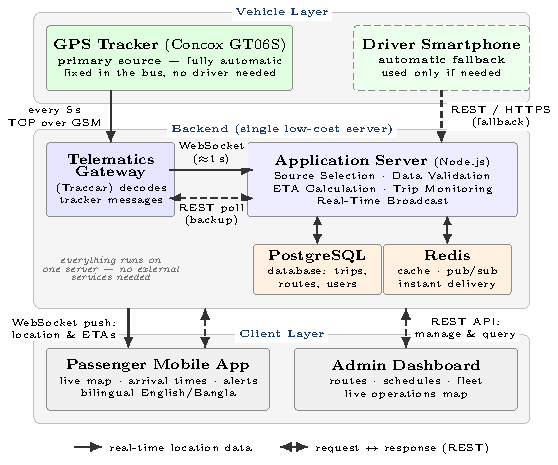
\includegraphics[page=1, width=0.9\textwidth]{twofigs.pdf}
\caption[System architecture of \system{}]{System architecture of
\system{}. The GPS tracker is the primary, fully automatic source; the
driver's smartphone is only a fallback. All backend components share one
low-cost server. Solid arrows carry real-time location data; dashed
double-headed arrows are REST request/response paths.}
\label{fig:arch}
\end{figure}

Three design decisions define the architecture:

\begin{enumerate}
  \item \textbf{Hardware-first acquisition.} The primary position source
  is a fixed, vehicle-grade tracker that operates with no human
  involvement. Anything a person must remember to do daily will
  eventually not be done; the design removes that failure mode entirely,
  and demotes the smartphone to an optional fallback
  (Section~\ref{sec:design-acquisition}).
  \item \textbf{A single low-cost server.} The application server,
  telematics gateway, database, and cache are co-hosted on one virtual
  private server. This satisfies NFR-3 and simplifies operations, while
  the Redis pub/sub back-plane preserves the option of scaling the
  realtime tier horizontally later (Section~\ref{sec:design-realtime}).
  \item \textbf{Event-driven processing.} Each arriving fix triggers a
  processing chain---arbitrate, filter, estimate, persist, publish---and
  everything downstream of the fix is pushed, never polled, so passenger
  latency is bounded by acquisition rather than by client refresh cycles.
\end{enumerate}

\section{Real-Time Data Flow}
\label{sec:design-flow}
Figure~\ref{fig:flow} traces the life of a single position report through
the system, grouped into three phases: acquisition (capture and
transmission), processing (arbitration, filtering, ETA computation), and
delivery (persistence, publication, and push). The seven steps of the
figure correspond to the design sections of this chapter and the
implementation sections of Chapter~\ref{ch:implementation}.

\begin{figure}[H]
\centering
\includegraphics[page=2, width=0.72\textwidth]{twofigs.pdf}
\caption[Real-time data flow]{Real-time data flow: the life of one
position report, from the GPS fix on the bus to the passenger's screen.
The timeline on the right shows representative latencies measured in the
pilot; the median end-to-end acquisition latency was 5.9\,s.}
\label{fig:flow}
\end{figure}

\section{GPS-Acquisition Layer}
\label{sec:design-acquisition}

\subsection{Primary Source: Fixed Vehicle Tracker}
The primary source is a Concox GT06S, a vehicle-grade GPS/GSM tracker
hard-wired to the bus's electrical system. While the vehicle moves, the
unit obtains a satellite fix every 5 seconds and transmits it over the
cellular network (TCP over GSM) to a self-hosted Traccar telematics
server, which implements the tracker's binary protocol and decodes each
message within about a second. Because the tracker is fixed to the
vehicle and powered from it, tracking requires no driver action, no
driver-owned device, and no driver data plan---the property on which the
whole operational-feasibility argument rests.

\subsection{Secondary Source: Driver Smartphone (Optional)}
A bus without a working tracker---not yet fitted, faulty, or SIM
depleted---can still be tracked. A driver smartphone running the app in
driver mode publishes its location to an authenticated REST endpoint.
This path is deliberately \emph{optional}: it exists so that coverage
degrades gracefully, not because the system depends on it. During the
pilot, two of the three buses were not yet fitted with trackers, so this
fallback path carried a substantial share of real trips
(Section~\ref{sec:eval-sources}).

\subsection{Ingesting from the Telematics Gateway}
The application server consumes Traccar's decoded positions through two
complementary paths, designed so that the faster one is used whenever
possible and the slower one guarantees delivery:

\begin{itemize}
  \item \textbf{Push (preferred).} A session-cookie WebSocket
  subscription to Traccar delivers each new fix within about one second
  of decoding.
  \item \textbf{Poll (backup).} A REST polling job queries Traccar every
  8 seconds during active trips, covering intervals when the socket is
  unavailable. (After the idle-efficiency optimization of
  Section~\ref{sec:eval-efficiency}, polling drops to every 60 seconds
  for buses with no active or imminent trip.)
\end{itemize}

\section{Source Arbitration Design}
\label{sec:design-arbitration}
When both a tracker and a driver phone are reporting for the same bus,
exactly one of them must drive the position passengers see. The design
maintains, per bus, one \emph{source-tracking state} for each active
source and a single \emph{canonical tracking state} for the public
position. On every inbound fix, an arbitration routine scores each
source's health---essentially its recency and validity---and selects the
canonical source by health and a configurable priority rank that prefers
the hardware tracker. Because the decision is re-evaluated per fix, a bus
can hand over from tracker to phone (or back) in the middle of a trip
with no passenger-visible artefact: the canonical marker simply continues
from the freshest healthy source. This satisfies FR-3 and NFR-2.

\section{Location-Quality Filtering Design}
\label{sec:design-filter}
Raw GPS cannot be displayed as-is. The design places a filtering pipeline
between arbitration and everything downstream, so that only credible
fixes can move the canonical position. Four operator-configurable rules
gate each fix:

\begin{enumerate}
  \item \textbf{Accuracy gate.} Fixes reporting accuracy worse than
  120\,m are soft-rejected; worse than 250\,m, hard-rejected.
  \item \textbf{Teleport guard.} A fix implying an inter-fix speed above
  120\,km/h is physically implausible on the pilot routes and is
  rejected.
  \item \textbf{Minimum-movement floor.} Displacements under 4\,m are
  treated as stationary, suppressing the GPS jitter that would otherwise
  make a parked bus wander on the map.
  \item \textbf{Freeze/release hysteresis.} Under sustained poor
  accuracy the marker is held still, and motion resumes only on a
  confident displacement, preventing oscillation at the accuracy
  boundary.
\end{enumerate}

The thresholds are deliberately conservative: 120\,km/h exceeds any
plausible bus speed on the pilot routes, and the 4\,m floor sits above
the tracker's typical urban scatter, so legitimate motion is never
suppressed. A short-window rolling average of accepted speeds is
maintained per trip and feeds the ETA estimator. Full HMM map matching
(Section~\ref{sec:lit-gps}) was considered and rejected: the buses follow
a small set of fixed routes, so projecting onto the known polyline
achieves the needed stability at a fraction of the cost.

\section{Arrival-Time Estimation Design}
\label{sec:design-eta}
The ETA estimator is geometric and training-free, chosen so the system
is fully functional from its first day of deployment
(Section~\ref{sec:lit-eta} explains why data-driven models were not an
option at cold start).

The route is first reduced to a cumulative along-path distance array over
its ordered stops. Each accepted fix is projected onto the nearest route
segment using a planar (local equirectangular) projection, which yields
the bus's \emph{progress} distance along the route and its cross-track
offset; the projection makes the estimate robust to lateral GPS error and
to the bus running slightly off the idealized polyline. For every stop
still ahead, the remaining distance is the difference between the stop's
cumulative distance and the bus's progress; dividing by an effective
speed yields that stop's ETA. The effective speed is the per-trip
rolling average when it is reliable ($\geq 5$\,km/h), otherwise a
configurable default of 20\,km/h. Each estimate carries a
\textsc{high}/\textsc{medium}/\textsc{low} confidence label derived from
the quality of the speed signal, so the interface can be honest about
uncertainty. A stop is marked \emph{reached} when the bus enters an
80\,m arrival radius, which triggers a stop-arrival event and, for
subscribed riders, a push notification (FR-9). The complete procedure is
given as Algorithm~\ref{alg:eta}.

\begin{algorithm}[H]
\caption{Estimating the ETA to every upcoming stop}
\label{alg:eta}
\begin{algorithmic}[1]
\Require current bus GPS fix; ordered route stops; recent average speed
\Ensure an ETA and a confidence label for each stop ahead
\State Compute each stop's distance from the route start (cumulative)
\State Project the bus fix onto the nearest route segment to find how far
  along the route it has travelled (its \emph{progress})
\If{recent average speed $\geq 5$\,km/h}
  \State $speed \gets$ recent average speed
\Else
  \State $speed \gets 20$\,km/h \Comment{fallback default}
\EndIf
\ForAll{stops ahead of the bus}
  \State $remaining \gets (\text{stop's distance}) - (\text{progress})$
  \State $\text{ETA} \gets remaining / speed$
\EndFor
\State Assign a confidence (High/Medium/Low) from the speed quality
\If{the nearest stop is within 80\,m}
  \State mark it reached and notify subscribed riders
\EndIf
\State \Return the ETA and confidence for every stop ahead
\end{algorithmic}
\end{algorithm}

\section{Trip Lifecycle Design}
\label{sec:design-lifecycle}
A trip is modelled as a state machine, shown in
Figure~\ref{fig:lifecycle}:
\textsc{planned} $\rightarrow$ \textsc{pre\_trip} $\rightarrow$
\textsc{running} $\rightarrow$ \textsc{ended}.

\begin{figure}[H]
\centering
\resizebox{\textwidth}{!}{%
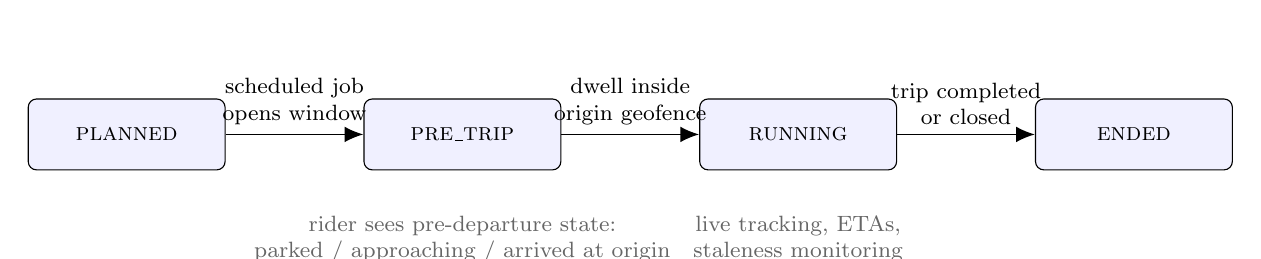
\begin{tikzpicture}[font=\small, node distance=1.75cm,
  st/.style={draw, rounded corners=3pt, fill=blue!6, minimum width=2.5cm,
             minimum height=9mm, align=center},
  ar/.style={-{Latex[length=2.4mm,width=2mm]}, semithick}]
\node[st] (pl) {\textsc{planned}};
\node[st, right=of pl] (pt) {\textsc{pre\_trip}};
\node[st, right=of pt] (ru) {\textsc{running}};
\node[st, right=of ru] (en) {\textsc{ended}};
\draw[ar] (pl) -- (pt) node[midway, above, font=\footnotesize, align=center]
  {scheduled job\\opens window};
\draw[ar] (pt) -- (ru) node[midway, above, font=\footnotesize, align=center]
  {dwell inside\\origin geofence};
\draw[ar] (ru) -- (en) node[midway, above, font=\footnotesize, align=center]
  {trip completed\\or closed};
\node[below=4.5mm of pt, font=\footnotesize, text=black!60, align=center]
  {rider sees pre-departure state:\\parked / approaching / arrived at origin};
\node[below=4.5mm of ru, font=\footnotesize, text=black!60, align=center]
  {live tracking, ETAs,\\staleness monitoring};
\end{tikzpicture}}%
\caption{The trip lifecycle state machine. The \textsc{pre\_trip} state is
what keeps the passenger's map informative before departure.}
\label{fig:lifecycle}
\end{figure}

The distinctive state is
\textsc{pre\_trip}: a scheduled job opens a window before the scheduled
departure during which the rider sees the bus's pre-departure state
---parked, approaching the origin, or arrived at the origin---instead of
a blank map (FR-7). The vehicle auto-promotes to \textsc{running} when it
dwells inside the origin geofence. A staleness job runs every 30 seconds
and flags any trip whose latest fix has aged beyond a threshold, so a
frozen marker is presented as \emph{stale} rather than silently passed
off as live (FR-8). Honesty about data age is treated as a first-class
interface requirement, not an afterthought.

\section{Database Design}
\label{sec:design-database}
PostgreSQL is the system of record, accessed through the Prisma ORM. The
schema comprises 31 relational models organized into six functional
domains, shown in Figure~\ref{fig:schema}.

\begin{figure}[H]
\centering
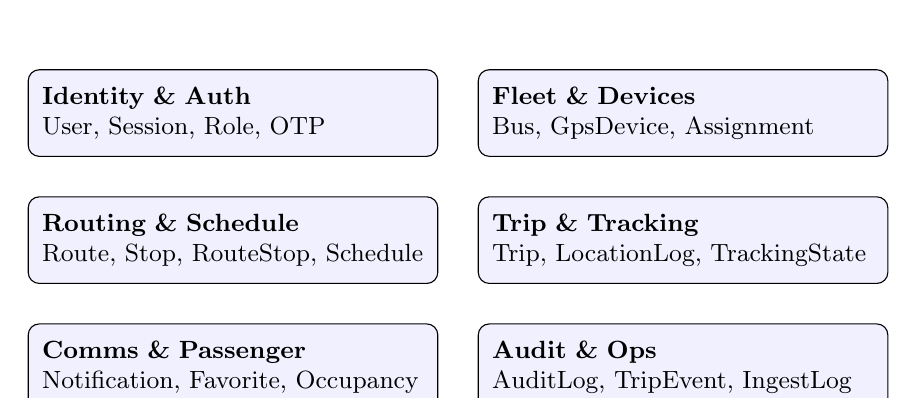
\begin{tikzpicture}[font=\small,
  dom/.style={draw, rounded corners, fill=blue!6, align=left,
              text width=0.40\textwidth, inner sep=5pt, minimum height=11mm}]
  \node[dom] (a) {\textbf{Identity \& Auth}\\User, Session, Role, OTP};
  \node[dom, right=5mm of a] (b) {\textbf{Fleet \& Devices}\\Bus, GpsDevice, Assignment};
  \node[dom, below=5mm of a] (c) {\textbf{Routing \& Schedule}\\Route, Stop, RouteStop, Schedule};
  \node[dom, right=5mm of c] (d) {\textbf{Trip \& Tracking}\\Trip, LocationLog, TrackingState};
  \node[dom, below=5mm of c] (e) {\textbf{Comms \& Passenger}\\Notification, Favorite, Occupancy};
  \node[dom, right=5mm of e] (f) {\textbf{Audit \& Ops}\\AuditLog, TripEvent, IngestLog};
\end{tikzpicture}
\caption{The 31-model relational schema, grouped into six functional
domains (representative models shown for each domain).}
\label{fig:schema}
\end{figure}

Two domains matter most to the thesis argument. \emph{Trip \& Tracking}
separates the per-source tracking states from the canonical tracking
state, which is what makes the arbitration design of
Section~\ref{sec:design-arbitration} expressible in data. \emph{Audit \&
Ops} preserves every raw ingest and trip event; this is the layer that
made the retrospective analysis of Chapter~\ref{ch:evaluation}---
including the discovery of the 98\% idle-reporting waste---possible
without any additional instrumentation.

\section{Realtime Delivery Design}
\label{sec:design-realtime}
Realtime delivery uses Socket.IO over WebSocket. Each active trip is a
logical \emph{room}; a passenger tracking a trip joins that trip's room
and thereafter receives only that trip's events, bounding per-client
traffic to the single vehicle being observed. Redis serves as the
publish/subscribe back-plane: accepted canonical updates and recomputed
ETAs are published once, and every server process holding subscribers for
that trip forwards them. This lets the realtime tier scale horizontally
without losing fan-out consistency (NFR-6), even though the pilot ran
comfortably on a single process. Authentication is enforced both at
socket connection and at room join (NFR-5).

Offline behaviour is part of the same design: the client retains the most
recent state, so a transient disconnection degrades to a ``last known''
view with an explicit staleness indicator rather than an empty screen.

\section{Security Design}
\label{sec:design-security}
All client--server traffic runs over HTTPS. Passengers and administrators
authenticate against the identity domain of the schema; role-based
authorization separates passenger, driver, and administrator
capabilities. The driver-side location endpoint accepts reports only from
an authenticated driver bound to the bus in question, preventing
arbitrary clients from injecting positions. Socket connections carry the
same identity, and room joins are authorized per trip. Administrative
actions are recorded in the audit domain.

\section{Summary}
This chapter presented the three-tier, event-driven architecture of
\system{} and the design of each major component: dual-source GPS
acquisition with per-fix health arbitration, the four-gate
location-quality filter, the training-free geometric per-stop ETA
estimator, the trip lifecycle with its pre-trip and staleness states,
the 31-model relational schema, the room-based realtime delivery layer,
and the security model. Chapter~\ref{ch:implementation} describes how
each design was realized.

% =====================================================================
\chapter{Implementation}
\label{ch:implementation}

\section{Backend Application Server}
\label{sec:impl-server}
The application server is written in TypeScript and runs on Node.js with
the Express framework. TypeScript was chosen over plain JavaScript
because the domain model is intricate---trips, sources, tracking states,
and their transitions---and static typing catches an entire class of
mistakes at compile time that would otherwise surface as runtime faults
on a live fleet.

Persistence goes through the Prisma ORM to PostgreSQL. Prisma generates
typed client code from the declarative schema, so a query that survives
compilation is structurally valid against the database. The 31 models of
the schema (Section~\ref{sec:design-database}) map one-to-one to Prisma
model declarations, and schema migrations are versioned alongside the
application code.

The server exposes two interfaces: a REST API (authentication, schedules,
routes, favourites, administration) and the Socket.IO realtime gateway.
Internally, the position-processing chain is implemented as a sequence of
services---ingestion, arbitration, filtering, ETA, publication---each of
which appends to the audit logs as it acts (FR-13).

\section{Traccar Integration}
\label{sec:impl-traccar}
A self-hosted Traccar instance decodes the Concox GT06S binary protocol.
The application server consumes it through the two paths designed in
Section~\ref{sec:design-acquisition}:

\begin{itemize}
  \item The \textbf{WebSocket push} path authenticates to Traccar with a
  session cookie and subscribes to its live position stream; a decoded
  fix reaches the application server within about one second.
  \item The \textbf{REST poll} path runs on a timer and reconciles the
  latest positions for all devices, guaranteeing progress when the
  socket is down. Its cadence is trip-aware: 8\,s for buses in an active
  trip or pre-trip window, 60\,s otherwise (the optimization of
  Section~\ref{sec:eval-efficiency}).
\end{itemize}

Every inbound fix---pushed, polled, or posted by a driver device---is
recorded with both its device-reported timestamp and its server-receipt
timestamp and tagged with its source. The difference between those two
timestamps is precisely the position-acquisition latency reported in
Chapter~\ref{ch:evaluation}, so the evaluation methodology was built into
the ingestion path from the start.

\section{Source Arbitration and Filtering}
\label{sec:impl-arbitration}
The arbitration routine of Section~\ref{sec:design-arbitration} runs on
every inbound fix. Health scoring is intentionally simple---recency and
validity dominate---because the failure mode it must detect is blunt: a
source going silent. The configurable priority rank prefers the hardware
tracker whenever it is healthy. During the pilot, mid-trip handovers
occurred and produced no passenger-visible discontinuity; the canonical
marker continued from the freshest healthy source, which is the exact
behaviour the design called for.

The filtering pipeline implements the four gates of
Section~\ref{sec:design-filter} with the thresholds listed in
Appendix~\ref{app:params} (accuracy soft/hard limits 120\,m/250\,m,
teleport guard 120\,km/h, movement floor 4\,m). Accepted fixes update the
canonical state, append to the per-trip location log, and refresh the
rolling speed window; rejected fixes are logged with their rejection
reason, which proved invaluable when tuning the thresholds early in the
pilot.

\section{ETA Computation}
\label{sec:impl-eta}
The estimator implements Algorithm~\ref{alg:eta} directly. Route geometry
is preprocessed once into a cumulative-distance array; per fix, the
projection and the per-stop loop are a few hundred floating-point
operations, so the estimator adds no measurable load even at full
reporting rate. Every prediction is logged with its trip, stop, predicted
instant, and confidence label, building the dataset against which
mean-absolute-error can be measured as arrivals accumulate---and from
which a learned predictor can later be trained
(Section~\ref{sec:concl-future}).

\section{Trip Lifecycle and Background Jobs}
\label{sec:impl-lifecycle}
Three scheduled jobs drive the lifecycle of
Section~\ref{sec:design-lifecycle}:

\begin{itemize}
  \item The \textbf{pre-trip job} opens the \textsc{pre\_trip} window
  ahead of each scheduled departure, computes the vehicle's
  pre-departure state (parked, approaching origin, arrived at origin),
  and promotes the trip to \textsc{running} when the bus dwells inside
  the origin geofence.
  \item The \textbf{staleness job} runs every 30\,s and flags trips whose
  latest fix has aged beyond the threshold, switching the passenger view
  to its explicit stale presentation.
  \item The \textbf{polling job} implements the trip-aware Traccar
  reconciliation cadence described above.
\end{itemize}

\section{Passenger Mobile Application}
\label{sec:impl-passenger}
The passenger application is built with React Native and Expo, targeting
Android first (the platform of essentially all pilot riders). Its
central screen is a live map showing the route polyline, its stops, and
the bus marker with a callout presenting the vehicle's label, next stop,
ETA, and current speed.

Four behaviours distinguish it from a naive tracker, each an edge
condition handled by design:

\begin{itemize}
  \item \textbf{Pre-trip awareness.} During the \textsc{pre\_trip}
  window the app renders the bus at its known pre-departure position
  (typically the depot or origin), so the map is never blank while a
  rider waits for departure (FR-7).
  \item \textbf{Staleness signalling.} When the server flags a trip
  stale, the app says so explicitly instead of letting a frozen marker
  masquerade as live data (FR-8).
  \item \textbf{Offline retention.} On a transient disconnection the app
  keeps the last known state visible, marked as such, and resumes
  seamlessly on reconnect.
  \item \textbf{Drop-off alerts.} A rider selects their stop; when the
  bus enters the 80\,m arrival radius, a push notification fires even if
  the app is backgrounded (FR-9), using a foreground location service
  for continued tracking.
\end{itemize}

The interface is fully bilingual. Every string in the application exists
in English and Bangla, switchable in-app at any time (FR-10), and place
names render in both scripts. Localization was implemented as a
first-class concern from the first screen onward---retrofitting
translation onto a finished English app tends to leave exactly the gaps
that erode user trust. Representative screens are shown in
Figure~\ref{fig:screens} (Appendix~\ref{app:screens} reproduces them at
full page width).

\begin{figure}[H]
\centering
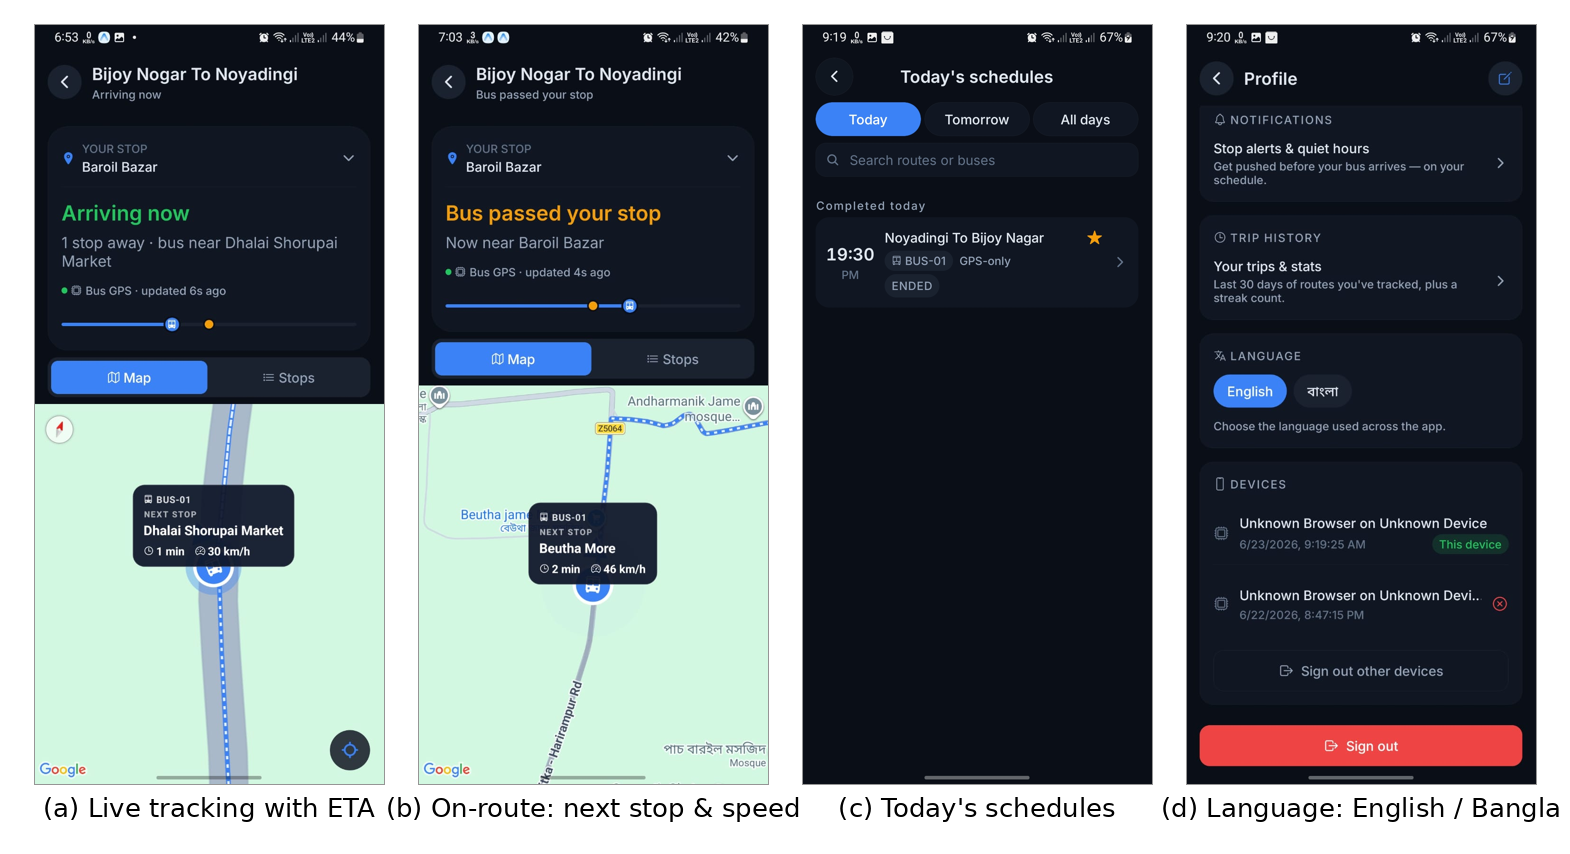
\includegraphics[width=\textwidth]{screens.png}
\caption[Screens of the bilingual passenger application]{The bilingual
passenger application. (a) live tracking of a moving bus with the
next-stop ETA; (b) on-route status showing the next stop and current
speed; (c) today's schedules; (d) the in-app English/Bangla language
toggle. Place names render in both scripts.}
\label{fig:screens}
\end{figure}

\section{Driver Mobile Application (Fallback Publisher)}
\label{sec:impl-driver}
The optional smartphone fallback of Section~\ref{sec:design-acquisition}
is served by a separate, purpose-built driver application (React Native
and Expo, distributed directly to drivers rather than publicly). It is
deliberately minimal---a login screen and a single home screen---because
its only job is to publish the bus position when a vehicle has no
working tracker. Figure~\ref{fig:driver} shows its principal states.

Four design decisions define it:

\begin{itemize}
  \item \textbf{Explicit sharing lifecycle.} The app shares nothing
  until the driver taps \emph{Start trip}, and stops the moment the
  trip ends; between trips it shows an explicit ``not sharing'' state.
  Location is therefore published only during an active trip.
  \item \textbf{Background publishing.} Unlike the passenger app, the
  driver app declares Android background-location permissions and runs
  a foreground service, with the publishing task registered at the
  global JavaScript scope so the operating system can invoke it even
  when the screen is off. Each fix is posted to the authenticated
  driver-location REST endpoint (FR-2), reading the active trip and
  credentials from secure storage.
  \item \textbf{Source selection in view.} The home screen carries the
  \emph{bus device / my phone} source selector and, while live, shows
  the driver the same telemetry the server sees---current speed, GPS
  accuracy, and seconds since the last update---so a driver can confirm
  at a glance that publishing is working.
  \item \textbf{Role guarding.} Only accounts with the driver role can
  proceed past login; any other account is refused inside the app.
\end{itemize}

\begin{figure}[H]
\centering
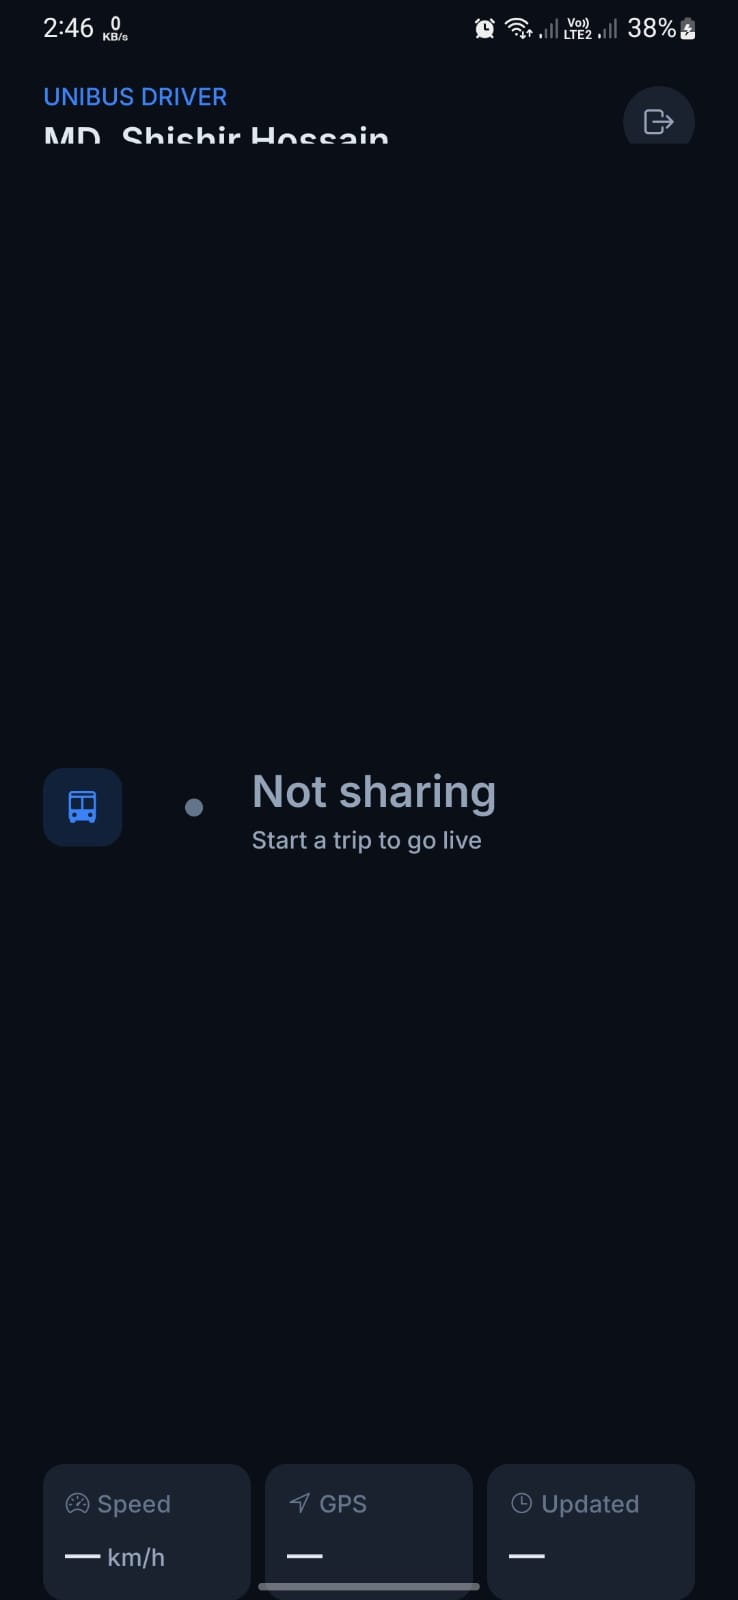
\includegraphics[width=0.235\textwidth]{driver_shots/idle.jpg}\hfill
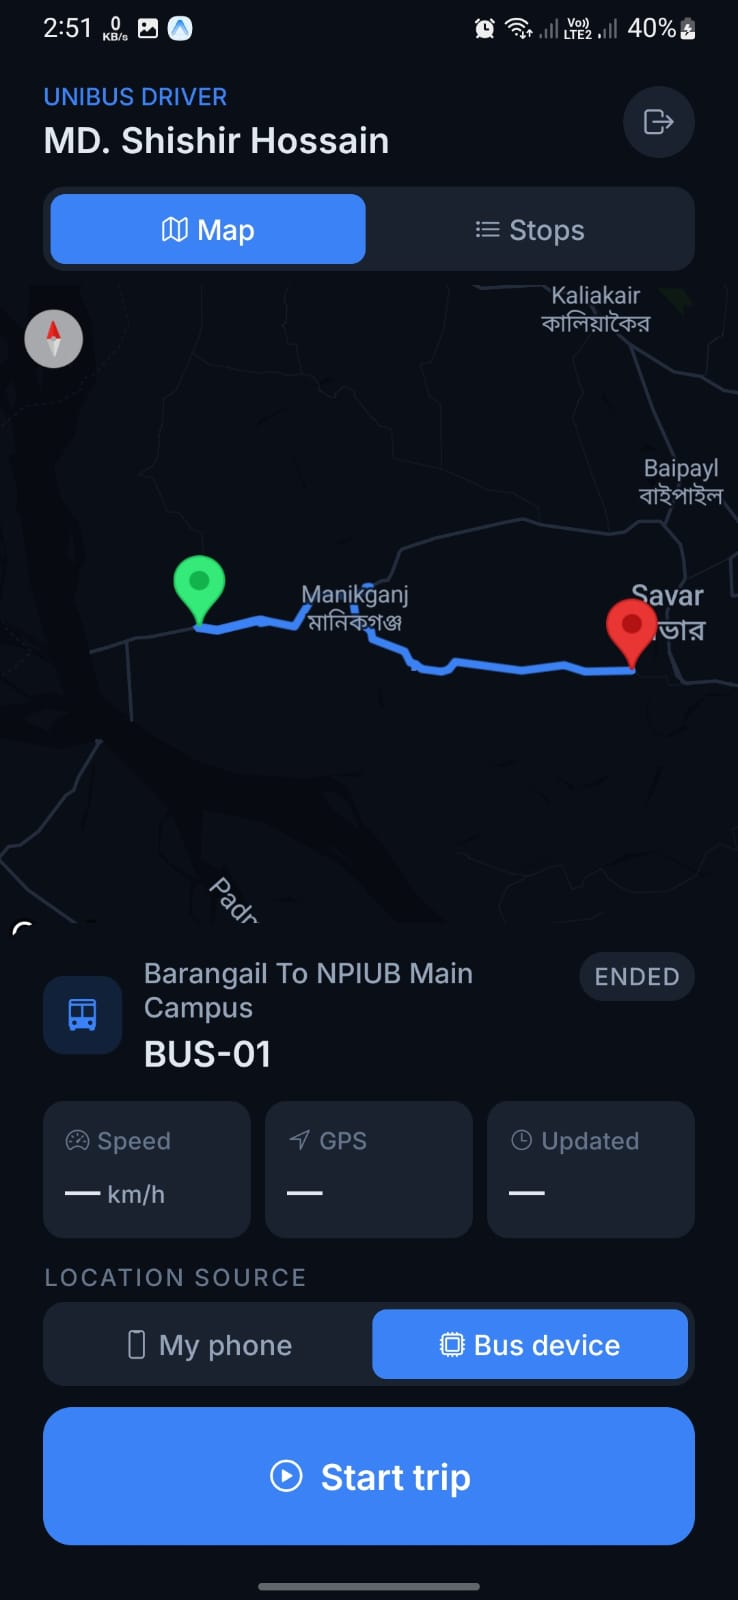
\includegraphics[width=0.235\textwidth]{driver_shots/routemap.jpg}\hfill
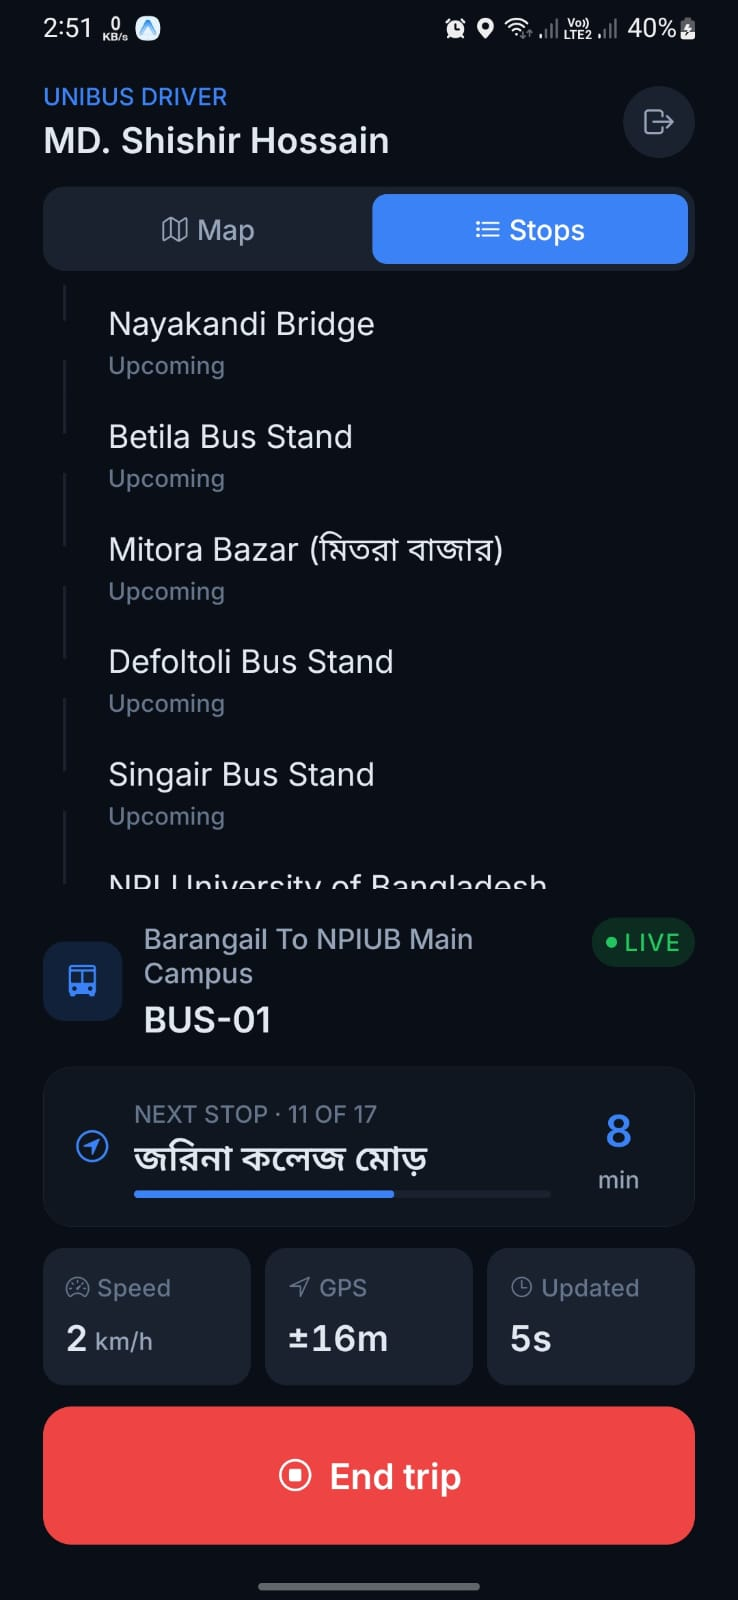
\includegraphics[width=0.235\textwidth]{driver_shots/live.jpg}\hfill

\includegraphics[width=0.235\textwidth]{driver_shots/stops.jpg}
\caption[Screens of the driver application]{The driver application.
Left to right: (a) the idle state---nothing is shared until a trip is
started; (b) the assigned trip's route map with the location-source
selector (bus device / my phone) and the \emph{Start trip} control;
(c) an active trip publishing \textsc{live}: next stop (11 of 17) with
its ETA, current speed, GPS accuracy, seconds since the last update,
and the \emph{End trip} control; (d) the stop-by-stop progress view
with done/next/upcoming states, stop names rendered in both scripts.}
\label{fig:driver}
\end{figure}

\section{Administration Console}
\label{sec:impl-admin}
The administration console is a server-rendered React application built
with Next.js. It integrates the Google Maps JavaScript API for two
map-centric tools: the \emph{live operations map}, which shows every
active vehicle in the fleet at once (FR-12), and the \emph{route
builder}, with which an administrator lays out a route's polyline and
stop sequence directly on the map. Figure~\ref{fig:admin} shows four of
its principal screens; Appendix~\ref{app:adminscreens} reproduces the
remaining management pages. Beyond the maps, the console manages
buses, GPS devices, schedules, and user roles through the same REST API
the mobile app uses (FR-11)---one API surface, two clients, no
duplicated logic.

\begin{figure}[H]
\centering
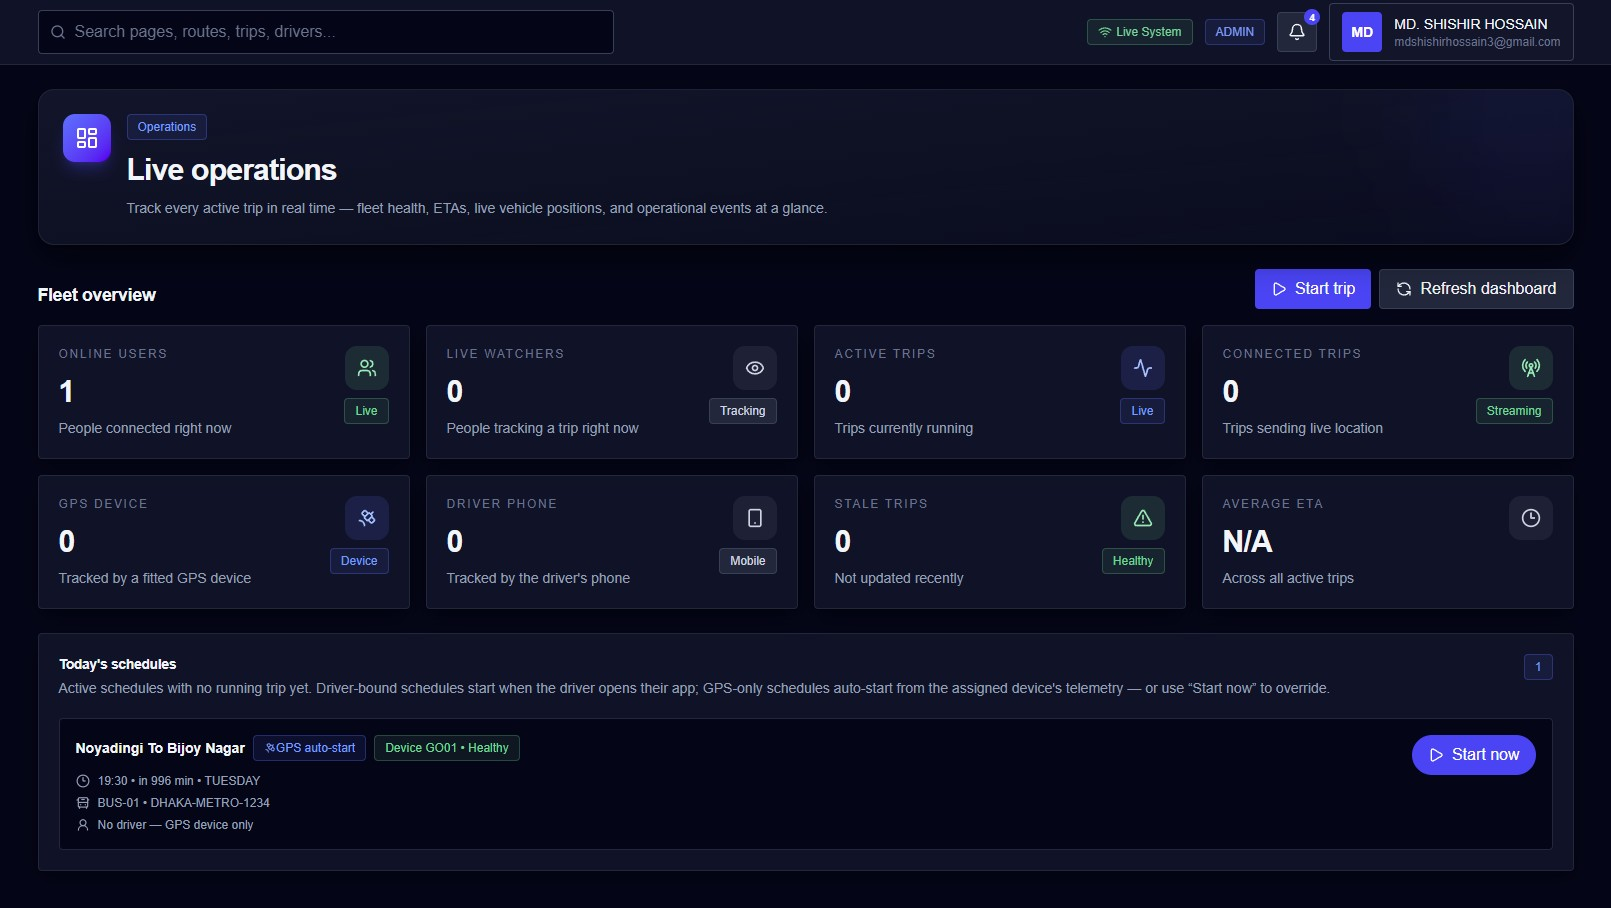
\includegraphics[width=0.49\textwidth]{admin/live_ops.jpg}\hfill
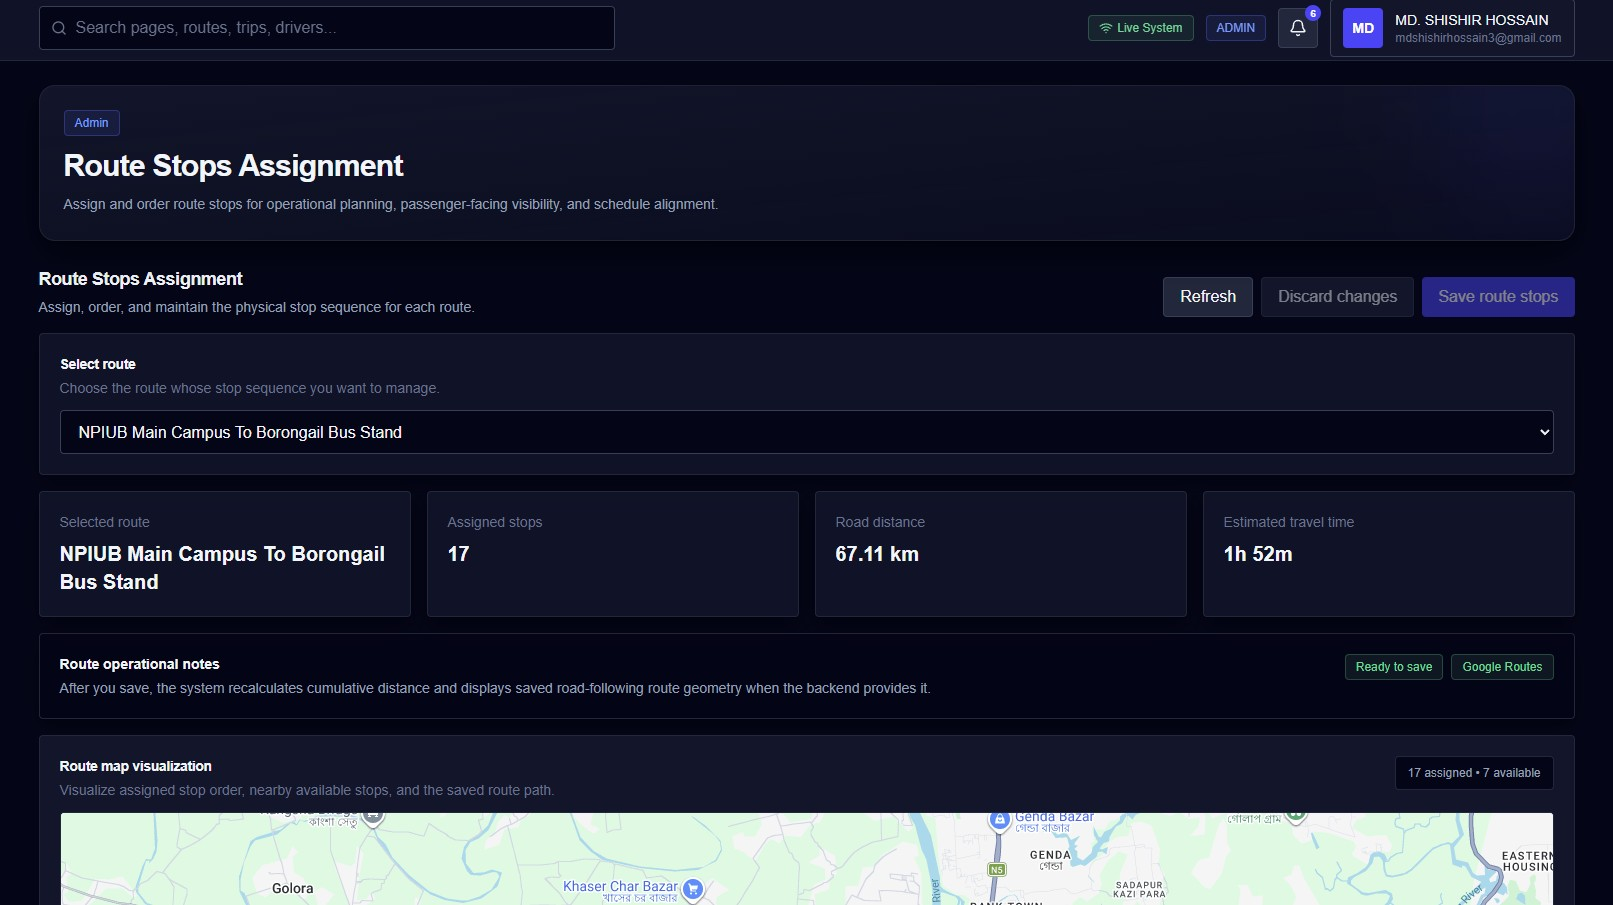
\includegraphics[width=0.49\textwidth]{admin/route_builder.jpg}\\[2mm]
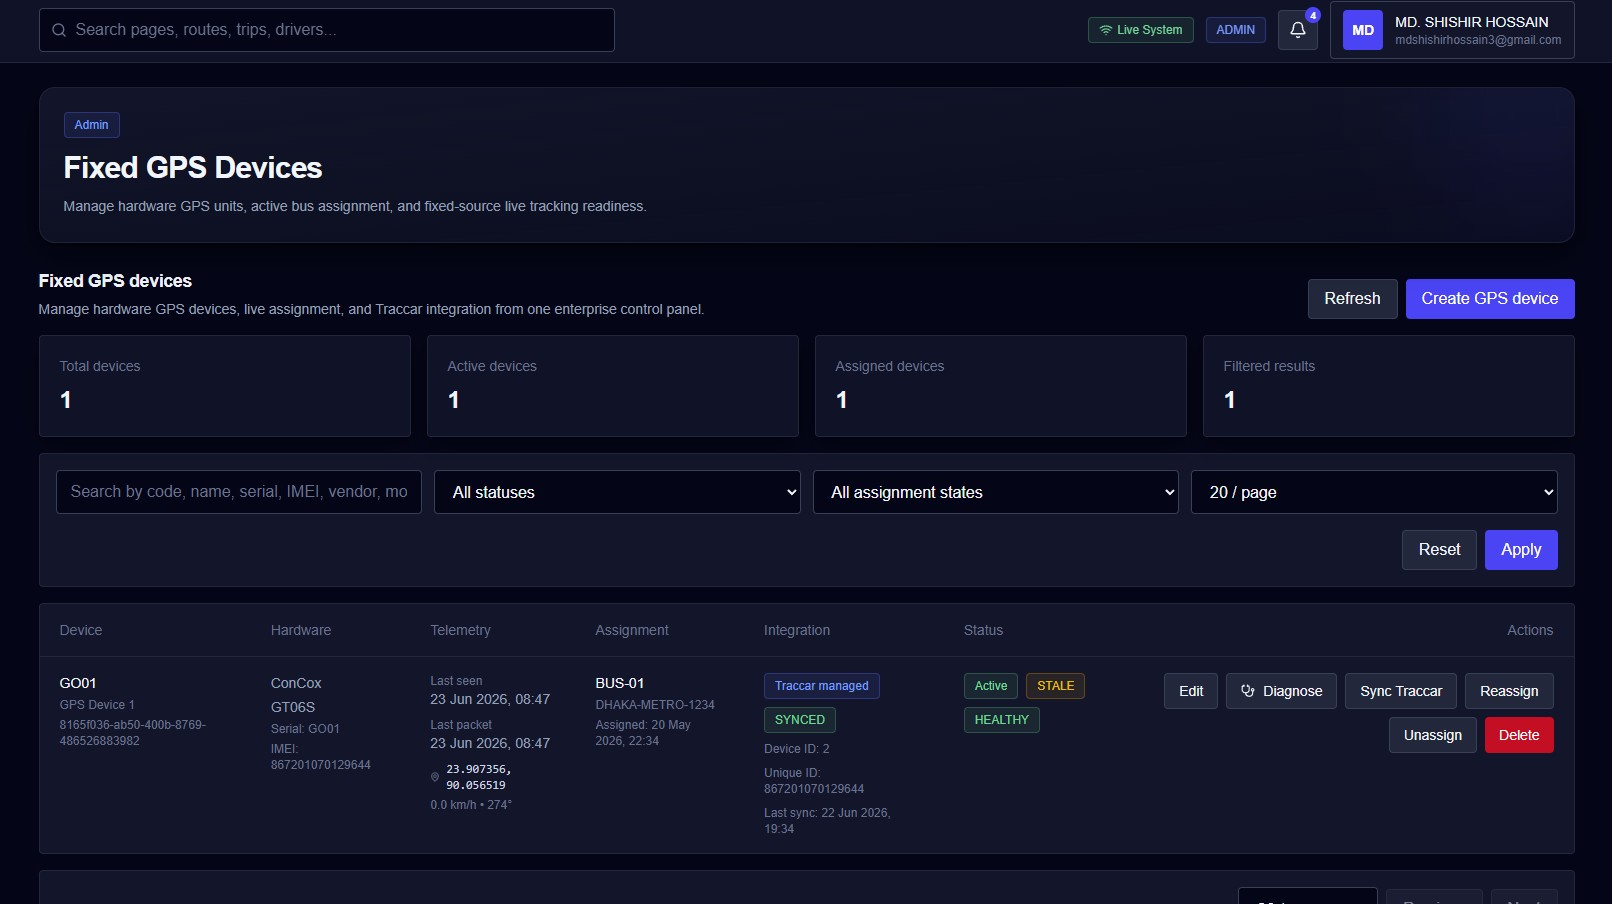
\includegraphics[width=0.49\textwidth]{admin/devices.jpg}\hfill
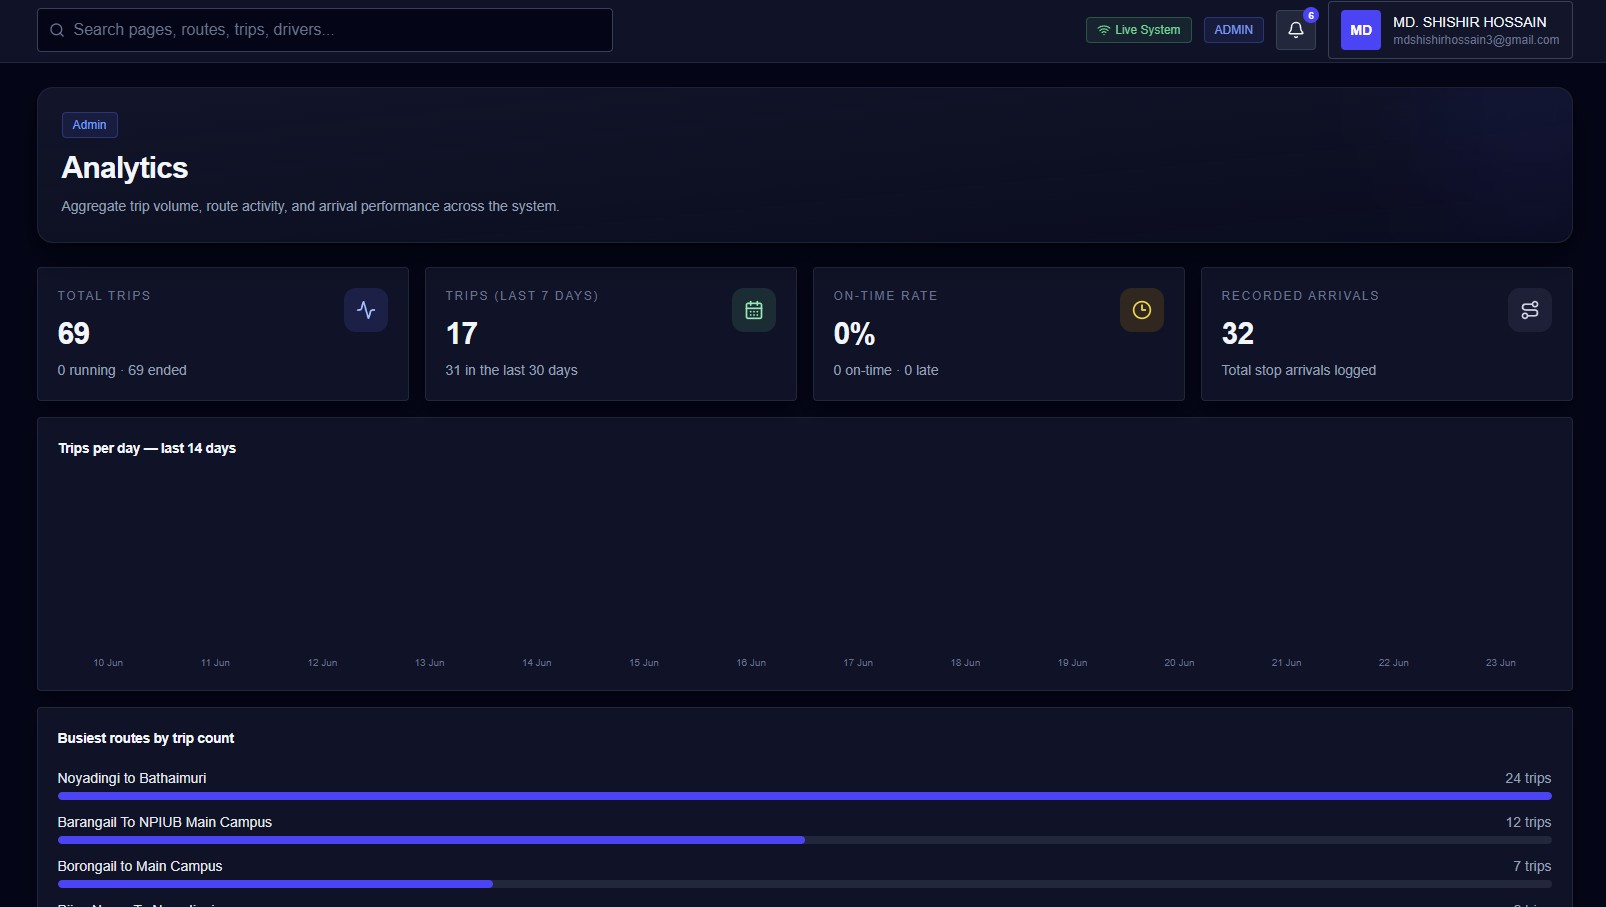
\includegraphics[width=0.49\textwidth]{admin/analytics.jpg}
\caption[Principal screens of the administration console]{Principal
screens of the administration console. Top left: the live operations
dashboard with the fleet overview and today's schedules. Top right: the
route-builder view, assigning the ordered stop sequence of a route with
its along-path distance, estimated travel time, and map visualization.
Bottom left: the fixed GPS device registry with telematics-integration
status and per-device diagnostics. Bottom right: the analytics view
aggregating trip volume, route activity, and arrival performance.}
\label{fig:admin}
\end{figure}

\section{On-Vehicle Device Configuration}
\label{sec:impl-device}
The Concox GT06S is configured over SMS, and its configuration became an
integral part of the system's efficiency story. The unit as initially
deployed transmitted a fix every 5 seconds \emph{regardless of vehicle
state}---including all night, parked in the depot. After the pilot data
quantified this waste (Section~\ref{sec:eval-efficiency}), we set an
asymmetric reporting cadence directly on the device:

\begin{itemize}
  \item \texttt{TIMER,5,300\#} --- report every 5\,s while moving, but
  only every 300\,s while static;
  \item \texttt{PARAM\#} --- read back the active configuration for
  verification;
  \item \texttt{STATUS\#} --- report battery and GSM/GPS state;
\end{itemize}

each acknowledged by return SMS (the full command set appears in
Appendix~\ref{app:sms}). We verified the change from two independent
vantage points---the per-position timestamps in Traccar's report view
and the server's own ingest log---confirming parked-state fixes spaced
by minutes rather than seconds, while a live test drive still produced
dense five-second fixes. A low-frequency heartbeat keeps the device
visible online between reports. Wiring the ignition (ACC) line for
engine-state-triggered sleep is identified as future work.

\section{Deployment}
\label{sec:impl-deploy}
The entire backend---application server, Traccar, PostgreSQL, and
Redis---runs on a single low-cost virtual private server, satisfying
NFR-3. The passenger application is distributed as an Android APK built
through the Expo Application Services build pipeline; the administration
console is served from the same VPS. No managed cloud services, message
queues, or third-party realtime providers are involved: the design goal
that a university could replicate this deployment for the cost of one
small server and one tracker per bus held from the first day of the
pilot to the last.

\section{Summary}
This chapter described the realization of the design: the TypeScript
application server and its typed persistence layer, the dual push/poll
Traccar integration with per-fix latency instrumentation, the
arbitration and filtering services, the direct implementation of the ETA
algorithm, the three lifecycle jobs, the bilingual passenger application
with its four edge-condition behaviours, the dedicated driver
application that implements the fallback publishing path, the
administration console, the SMS-based tracker configuration, and the
single-server deployment. The next chapter evaluates the deployed whole
on the real fleet.

% =====================================================================
\chapter{Testing, Results and Evaluation}
\label{ch:evaluation}

\section{Testing Approach}
\label{sec:eval-testing}
The system was verified at four levels before and during the pilot, in
keeping with the iterative methodology of Chapter~\ref{ch:analysis}:

\begin{description}
  \item[Static verification.] The entire server and mobile codebase is
  written in TypeScript and kept free of type errors; the Prisma ORM
  extends this guarantee to the database boundary, since queries are
  type-checked against the 31-model schema at compile time.
  \item[Component verification.] Each pipeline stage was exercised
  against live data as it was added. The filtering thresholds in
  particular were tuned empirically: rejected fixes are logged with
  their rejection reason (Section~\ref{sec:impl-arbitration}), and
  reviewing those logs during early deployment confirmed that the gates
  rejected genuine noise---urban scatter, impossible jumps---without
  suppressing legitimate motion.
  \item[End-to-end verification on the road.] The complete chain---GPS
  fix, cellular transmission, decoding, arbitration, filtering, ETA,
  push, and on-screen rendering---was verified with live test drives on
  the actual routes, observing the passenger application against the
  visible position of the real bus. Device-configuration changes were
  verified from two independent vantage points (Traccar's report view
  and the server's ingest log, Section~\ref{sec:impl-device}).
  \item[Continuous operational verification.] Because every layer logs
  (FR-13), the running pilot itself acted as a seven-week continuous
  test: anomalies surfaced in the audit data rather than in user
  reports, which is also how the idle-reporting problem of
  Section~\ref{sec:eval-efficiency} was found.
\end{description}

\section{Pilot Deployment and Dataset}
\label{sec:eval-dataset}
\system{} was evaluated in a seven-week pilot, from 6~May to
23~June~2026, on the operational university fleet---real buses, real
routes, real riders, zero simulation. The deployment covered 9 routes
and 3 buses, one of which was equipped with the fixed hardware tracker;
38 passenger accounts were registered, and 71 completed trips were
recorded, during which 46{,}548 raw GPS reports were ingested.
Table~\ref{tab:dataset} summarizes the dataset.

\begin{table}[H]
\caption{Pilot deployment summary.}
\label{tab:dataset}
\centering
\begin{tabular}{@{}lr@{}}
\toprule
\textbf{Quantity} & \textbf{Value} \\
\midrule
Deployment span            & 7 weeks (6 May -- 23 June 2026) \\
Routes                     & 9 \\
Buses                      & 3 (1 fitted with hardware tracker) \\
Registered passengers      & 38 \\
Completed trips            & 71 \\
Raw GPS reports ingested   & 46{,}548 \\
In-trip fixes retained     & 864 \\
Mean GPS fixes per trip    & 37.6 \\
\bottomrule
\end{tabular}
\end{table}

One number in Table~\ref{tab:dataset} demands immediate attention: of
46{,}548 raw reports, only 864 were retained as in-trip fixes. The
remaining ${\sim}98\%$ were transmitted while buses were parked. This
single observation---invisible during design, unmistakable in the
operational data---motivated the efficiency optimization analysed in
Section~\ref{sec:eval-efficiency}, and is in our view one of the most
instructive findings of the whole project.

\section{Measurement Methodology}
\label{sec:eval-method}
All metrics are computed from the production database; no separate test
harness or synthetic workload was used. Position-acquisition latency is
the difference between each fix's device-reported timestamp and its
server-receipt timestamp, both recorded at ingestion
(Section~\ref{sec:impl-traccar}). Source usage is taken from the
canonical source selected per trip. Passenger engagement is measured
from the notification delivery and read records. ETA accuracy is
assessed through the prediction log: every predicted arrival instant is
retained so it can be compared against the corresponding recorded stop
arrival. Because the pilot is small, we report results as a feasibility
demonstration rather than as population statistics.

\section{Results}

\subsection{Position-Acquisition Latency}
\label{sec:eval-latency}
Across 46{,}286 fixes with valid timestamp pairs, the latency from
device fix to server receipt was:

\begin{table}[H]
\caption{Position-acquisition latency (device fix to server receipt).}
\label{tab:latency}
\centering
\begin{tabular}{@{}lr@{}}
\toprule
\textbf{Statistic} & \textbf{Latency} \\
\midrule
Median            & 5.9\,s \\
Mean              & 7.4\,s \\
90th percentile   & 9.9\,s \\
95th percentile   & 11.1\,s \\
\bottomrule
\end{tabular}
\end{table}

A further median 1.2\,s elapsed between server receipt and persistence.
The latency distribution is bounded primarily by the 8\,s Traccar
polling interval rather than by network transport: when the WebSocket
push path is active a fix arrives within about a second, and the polling
path fills the remainder of the distribution. For the passenger this
means the map reflects reality within roughly six seconds in the median
case---comfortably inside the ``live'' perception window for a vehicle
that takes minutes between stops (NFR-1 satisfied).

\subsection{Source Resilience}
\label{sec:eval-sources}
The dual-source design was exercised in earnest rather than remaining a
theoretical safeguard. Of the 70 trips with a recorded canonical source,
45 (64\%) were tracked via the fixed hardware tracker and 25 (36\%) via
the smartphone fallback. The fallback share largely reflects the two
buses not yet fitted with trackers---exactly the deployment reality the
fallback was designed for. Coverage was sustained across the whole
fleet throughout the pilot even though only one bus carried hardware.

Two readings follow. First, graceful degradation works: a bus without a
tracker remained trackable, and mid-trip handovers produced no
passenger-visible artefacts. Second, the design remains hardware-first:
the tracker operates with no driver involvement, and as trackers are
fitted fleet-wide the smartphone path reduces to a rarely needed safety
net (NFR-2 satisfied).

\subsection{ETA Estimation Behaviour}
\label{sec:eval-eta}
The geometric estimator produced a per-stop arrival prediction on every
accepted fix, each carrying its \textsc{high}/\textsc{medium}/\textsc{low}
confidence label. Every prediction was logged against its trip and stop,
so mean absolute error against recorded stop arrivals can be measured
cumulatively as operational data grows. Within the pilot itself the
prediction log was validated end-to-end (predictions recorded, arrivals
recorded, joinable per stop); a statistically meaningful MAE requires
more arrivals per stop than seven weeks provided, and is deliberately
reported as accumulating future evidence rather than overstated from
sparse data.

\subsection{Passenger Engagement}
\label{sec:eval-engagement}
Of 45 arrival and service notifications delivered to riders during the
pilot, 36 (80\%) were read. For a passive daily-utility application this
read rate indicates that the alerts were genuinely attended to rather
than dismissed as noise, supporting the design decision to invest in
proximity-based drop-off alerts (FR-9).

\section{The Idle-Reporting Problem and Optimization}
\label{sec:eval-efficiency}
This section analyses the pilot's most consequential finding.

\subsection{The Discovery}
The fixed-interval tracker transmitted a fix every 5 seconds whenever it
was powered---and it is wired to the vehicle battery, so it was always
powered. Buses, however, spend most of their day parked. The result, in
plain numbers: of 46{,}548 raw reports, only 864 fell inside any active
trip. Roughly \textbf{98\% of all transmissions were waste}---consuming
cellular data on the tracker's SIM, drawing on the bus battery, and
occupying server ingestion for positions nobody would ever look at.

Nothing in the design phase predicted this, because each individual
report is cheap; only the operational aggregate exposed the cost. This
is precisely the kind of finding that distinguishes a deployed
evaluation from a simulation.

\subsection{The Two-Sided Fix}
The waste was attacked at both ends of the pipeline:

\begin{itemize}
  \item \textbf{Device side.} The tracker was reconfigured over SMS
  (\texttt{TIMER,5,300\#}, Section~\ref{sec:impl-device}) to an
  asymmetric cadence: every 5\,s while moving, every 300\,s while
  static---a $60\times$ reduction in parked-state transmissions at the
  source, saving cellular data and battery on the vehicle itself.
  \item \textbf{Server side.} The Traccar polling job was made
  trip-aware: full-rate 8\,s polling now applies only to buses in an
  active trip or pre-trip window, while idle buses are polled every
  60\,s---a $7.5\times$ reduction in idle polling, leaving the WebSocket
  push path and on-trip tracking untouched.
\end{itemize}

\begin{table}[H]
\caption{Idle-reporting efficiency optimization.}
\label{tab:efficiency}
\centering
\begin{tabular}{@{}llrrr@{}}
\toprule
\textbf{Layer} & \textbf{Parameter} & \textbf{Before} & \textbf{After}
& \textbf{Reduction} \\
\midrule
Device (GT06S) & Parked report interval & 5\,s & 300\,s & $60\times$ \\
Server         & Idle poll interval     & 8\,s & 60\,s  & $7.5\times$ \\
\bottomrule
\end{tabular}
\end{table}

\subsection{Verification}
The device-side change was verified from two independent vantage
points: the per-position timestamps in Traccar's report view, and the
server's own ingest log. Both showed parked-state fixes spaced by
minutes rather than seconds after the change, while a live test drive
confirmed that motion still produced dense five-second fixes---that is,
the optimization removed only the redundant reports, not the live
tracking (NFR-4 satisfied). After the optimization the server ingests
essentially only the dense fixes of active trips plus a sparse
five-minute parked heartbeat per bus, in place of the previous
continuous five-second stream.

\section{Requirements Coverage}
Table~\ref{tab:coverage} closes the loop between
Chapter~\ref{ch:analysis} and the pilot.

\begin{table}[H]
\caption{Requirements coverage demonstrated in the pilot.}
\label{tab:coverage}
\centering
\small
\begin{tabular}{@{}lp{10.6cm}@{}}
\toprule
\textbf{Req.} & \textbf{Pilot evidence} \\
\midrule
FR-1--FR-3 & 64\%/36\% tracker/fallback split across 70 sourced trips;
mid-trip handovers without artefacts. \\
FR-4 & Rejected fixes logged with reasons; displayed positions stable
throughout. \\
FR-5 & Per-stop ETA with confidence on every accepted fix; all
predictions logged. \\
FR-6 & Median 5.9\,s acquisition latency; push delivery on every
accepted update. \\
FR-7, FR-8 & Pre-trip vehicle state shown before departure; staleness
flagged within 30\,s. \\
FR-9 & 45 notifications delivered; 80\% read. \\
FR-10 & All pilot riders used the bilingual interface; both scripts
rendered. \\
FR-11--FR-12 & 9 routes, 3 buses, and all schedules administered through
the console. \\
FR-13 & Entire evaluation computed from production logs alone. \\
NFR-1--NFR-7 & Addressed respectively in
Sections~\ref{sec:eval-latency}, \ref{sec:eval-sources},
\ref{sec:impl-deploy}, \ref{sec:eval-efficiency},
\ref{sec:design-security}, \ref{sec:design-realtime},
and \ref{sec:impl-passenger}. \\
\bottomrule
\end{tabular}
\end{table}

\section{Limitations}
\label{sec:eval-limitations}
The results must be read with the pilot's boundaries in mind. The scale
is small---seven weeks, 3 buses, 38 riders---and a subset of trips were
operational tests. Only one bus carried the hardware tracker, so the
64/36 source split reflects fleet hardware coverage as much as tracker
reliability. The GT06S does not report a per-fix accuracy value, so
quality filtering is evaluated at the trip level rather than per fix.
Schedule-adherence analysis was limited by incomplete timetable
association during the pilot. The findings therefore demonstrate
feasibility; they do not claim city-scale statistical generality.

% =====================================================================
\chapter{Conclusion and Future Work}
\label{ch:conclusion}

\section{Conclusion}
This thesis set out to answer a practical question: can a university in
a developing region give its students live, trustworthy, in-their-own-
language information about their bus, at a cost the institution can
actually sustain? The answer, demonstrated on a real fleet rather than
in simulation, is yes.

We designed, implemented, and deployed \system{}, a complete real-time
bus tracking platform comprising a bilingual passenger mobile
application, a web administration console, and a central application
server backed by a 31-model relational schema---all self-hosted on a
single low-cost server. Its distinguishing technical ideas are:

\begin{itemize}
  \item \textbf{Resilient dual-source acquisition.} A fixed,
  vehicle-grade GPS tracker provides fully automatic, driver-independent
  positioning as the primary source, while the driver's smartphone
  serves only as an optional fallback, selected per fix by health-based
  arbitration. In the pilot this was no theoretical safeguard: 64\% of
  trips ran on hardware and 36\% on the fallback, sustaining coverage
  while most of the fleet awaited tracker installation.
  \item \textbf{A training-free geometric ETA estimator.} Projecting the
  live position onto the route polyline and dividing remaining distance
  by a rolling-average speed yields a per-stop arrival estimate with a
  confidence label from the first day of deployment, with every
  prediction logged for future learning-based refinement.
  \item \textbf{An edge-condition-aware passenger experience.} Pre-trip
  vehicle awareness, explicit staleness signalling, offline retention,
  and proximity-based drop-off alerts keep the interface honest and
  informative precisely where naive trackers show a blank or frozen
  map---in both English and Bangla.
\end{itemize}

The seven-week pilot on the operational fleet (9 routes, 3 buses, 38
riders, 71 trips, 46{,}548 GPS reports) established feasibility with a
median position-acquisition latency of 5.9\,s and an 80\% read rate on
delivered notifications. Just as importantly, the pilot taught a lesson
that no simulation would have: roughly 98\% of raw device reports were
redundant idle-state transmissions. The resulting two-sided
optimization---asymmetric device reporting (5\,s moving / 300\,s
parked) and trip-aware server polling (8\,s active / 60\,s idle)---cut
idle-period reporting by up to $60\times$ while leaving live tracking
untouched, and stands as a concrete, transferable design guideline for
any scheduled-fleet tracking deployment: \emph{couple reporting cadence
to vehicle state and timetable, at both the device and the server.}

\section{Future Work}
\label{sec:concl-future}
The deployed system and its accumulating operational data open several
concrete directions:

\begin{enumerate}
  \item \textbf{Learning-based ETA prediction.} Every prediction and
  every arrival is already logged. Once the trajectory history is large
  enough, a data-driven model (Section~\ref{sec:lit-eta}) can be trained
  and evaluated directly against the geometric baseline on the same
  logged data.
  \item \textbf{Fleet-wide tracker installation.} Fitting the remaining
  buses reduces the smartphone path to a rarely needed safety net and
  enables uniform fleet analytics.
  \item \textbf{Ignition-coupled reporting.} Wiring the tracker's ACC
  line would let the device sleep with the engine, completing the
  efficiency work of Section~\ref{sec:eval-efficiency} with
  engine-state-triggered reporting and distance-based thresholds.
  \item \textbf{Full timetable integration.} Associating every trip with
  its scheduled departure enables systematic schedule-adherence
  analytics for the transport office---the administrative counterpart of
  the passenger-facing ETAs.
  \item \textbf{Crowd-sourced occupancy.} At larger scale, passenger
  participation could add ``how full is the bus'' to ``where is the
  bus,'' complementing rather than carrying the positioning system.
  \item \textbf{A formal usability study.} A wider, longer deployment
  with a structured passenger study would quantify the experience
  benefits that the pilot's 80\% notification read rate only hints at.
\end{enumerate}

\section{Closing Remark}
The deepest lesson of this project is methodological. The system's most
valuable finding---the 98\% idle-reporting waste---was not visible in
any design document, simulator, or code review. It appeared only in the
operational data of a real deployment, and once visible, it was fixable
within days. Building the audit layer first, deploying early, and
letting production data drive the engineering agenda turned a student
project into an evaluated system; we commend the same path to those who
follow.


% =====================================================================
%                          REFERENCES
% =====================================================================
\clearpage
\addcontentsline{toc}{chapter}{References}
% =====================================================================
% REFERENCES (IEEE style, numbered to match in-text [n] citations)
% =====================================================================
\chapter*{References}
\markboth{References}{}

\begin{enumerate}[label={[\arabic*]}, leftmargin=1.2cm, itemsep=6pt]
  \item S.~A. Sharif, M.~S.~A. Suhaimi, N.~N. Jamal, I.~K. Riadz,
  I.~F. Amran, and D.~N.~A. Jawawi, ``Real-time campus university bus
  tracking mobile application,'' in \emph{Proc. 7th ICT International
  Student Project Conference (ICT-ISPC)}, 2018.

  \item K.~Premkumar, K.~Pavithra, J.~Presiela, D.~Priyadarshini, and
  P.~Priyanga, ``College bus tracking and notification system,'' in
  \emph{Proc. International Conference on System, Computation, Automation
  and Networking (ICSCAN)}, 2020.

  \item P.~Zhou, Y.~Zheng, Z.~Li, M.~Li, and G.~Shen, ``How long to wait?
  Predicting bus arrival time with mobile phone based participatory
  sensing,'' in \emph{Proc. 10th ACM International Conference on Mobile
  Systems, Applications, and Services (MobiSys)}, 2012.

  \item P.~Wepulanon, A.~Sumalee, and W.~H.~K. Lam, ``A real-time bus
  arrival time information system using crowdsourced smartphone data: a
  novel framework and simulation experiments,'' \emph{Transportmetrica B:
  Transport Dynamics}, vol.~6, no.~1, 2018.

  \item T.~Reich, M.~Budka, D.~Robbins, and D.~Hulbert, ``Survey of ETA
  prediction methods in public transport networks,'' \emph{arXiv preprint
  arXiv:1904.05037}, 2019.

  \item N.~Singh and K.~Kumar, ``A review of bus arrival time prediction
  using artificial intelligence,'' \emph{WIREs Data Mining and Knowledge
  Discovery}, vol.~12, no.~4, p.~e1457, 2022.

  \item L.~Ye and P.~Thiengburanathum, ``A real-time bus arrival time
  prediction system based on Spark framework and machine learning
  approaches: a case study in Chiang Mai,'' in \emph{Proc. Joint
  International Conference on Digital Arts, Media and Technology (ECTI
  DAMT \& NCON)}, 2020.

  \item N.~Rashvand, S.~S. Hosseini, M.~Azarbayjani, and H.~Tabkhi,
  ``Real-time bus arrival prediction: a deep learning approach for
  enhanced urban mobility,'' \emph{arXiv preprint arXiv:2303.15495},
  2023.

  \item N.~Rashvand, M.~Azarbayjani, S.~S. Hosseini, and H.~Tabkhi,
  ``Real-time bus departure prediction using neural networks for smart
  IoT public bus transit,'' \emph{IoT}, vol.~5, no.~4, pp.~650--665,
  2024.

  \item S.~Jeong, C.~Oh, and J.~Jeong, ``BAT-Transformer: prediction of
  bus arrival time with transformer encoder for smart public
  transportation system,'' \emph{Applied Sciences}, vol.~14, no.~20,
  art.~9488, 2024.

  \item R.~Barnes, S.~Buthpitiya, J.~Cook, A.~Fabrikant, A.~Tomkins, and
  F.~Xu, ``BusTr: Predicting bus travel times from real-time traffic,''
  in \emph{Proc. 26th ACM SIGKDD International Conference on Knowledge
  Discovery \& Data Mining (KDD)}, 2020, pp.~3243--3251.

  \item P.~Newson and J.~Krumm, ``Hidden Markov map matching through
  noise and sparseness,'' in \emph{Proc. 17th ACM SIGSPATIAL
  International Conference on Advances in Geographic Information
  Systems}, 2009, pp.~336--343.

  \item Traccar, ``Traccar: Open source GPS tracking platform.''
  [Online]. Available: \url{https://www.traccar.org/}

  \item OpenJS Foundation, ``Node.js.'' [Online]. Available:
  \url{https://nodejs.org/}

  \item OpenJS Foundation, ``Express: Fast, unopinionated, minimalist
  web framework for Node.js.'' [Online]. Available:
  \url{https://expressjs.com/}

  \item Prisma Data, Inc., ``Prisma ORM.'' [Online]. Available:
  \url{https://www.prisma.io/}

  \item PostgreSQL Global Development Group, ``PostgreSQL: The world's
  most advanced open source relational database.'' [Online]. Available:
  \url{https://www.postgresql.org/}

  \item Redis Ltd., ``Redis.'' [Online]. Available:
  \url{https://redis.io/}

  \item Socket.IO, ``Socket.IO: Bidirectional and low-latency
  communication for every platform.'' [Online]. Available:
  \url{https://socket.io/}

  \item Meta Platforms, Inc., ``React Native: Learn once, write
  anywhere.'' [Online]. Available: \url{https://reactnative.dev/}

  \item Expo, ``Expo: Create universal native apps with React.''
  [Online]. Available: \url{https://expo.dev/}

  \item Vercel, Inc., ``Next.js: The React framework.'' [Online].
  Available: \url{https://nextjs.org/}

  \item E.~D. Kaplan and C.~J. Hegarty, Eds., \emph{Understanding
  GPS/GNSS: Principles and Applications}, 3rd~ed. Norwood, MA, USA:
  Artech House, 2017.

  \item I.~Fette and A.~Melnikov, ``The WebSocket Protocol,'' IETF
  RFC~6455, Dec. 2011.
\end{enumerate}


% =====================================================================
%                          APPENDICES
% =====================================================================
\appendix
% =====================================================================
% APPENDICES
% =====================================================================

\chapter{Tracker SMS Configuration Commands}
\label{app:sms}
The Concox GT06S tracker is configured entirely over SMS; each command
is acknowledged by a return SMS from the device. Table~\ref{tab:sms}
lists the commands used during deployment and the pilot.

\begin{table}[H]
\caption{GT06S SMS commands used in this work.}
\label{tab:sms}
\centering
\small
\begin{tabular}{@{}lp{9.6cm}@{}}
\toprule
\textbf{Command} & \textbf{Effect} \\
\midrule
\texttt{TIMER,5,300\#} & Set asymmetric reporting: every 5\,s while the
vehicle is moving, every 300\,s while static. This is the device-side
half of the idle-efficiency optimization
(Section~\ref{sec:eval-efficiency}). \\
\texttt{PARAM\#} & Read back the active configuration, used to verify
that the \texttt{TIMER} change was applied. \\
\texttt{STATUS\#} & Report battery level and GSM/GPS state, used for
routine health checks during the pilot. \\
\bottomrule
\end{tabular}
\end{table}

The device also emits a low-frequency heartbeat between position
reports, which keeps it visible as \emph{online} to the telematics
server while parked.

\chapter{Operator-Configurable Processing Parameters}
\label{app:params}
Table~\ref{tab:params} consolidates the tunable parameters of the
position-processing pipeline with the values used in the pilot. All are
operator-configurable without code changes.

\begin{table}[H]
\caption{Pipeline parameters and pilot values.}
\label{tab:params}
\centering
\small
\begin{tabular}{@{}lll@{}}
\toprule
\textbf{Parameter} & \textbf{Pilot value} & \textbf{Role} \\
\midrule
Accuracy soft-reject      & 120\,m      & Quality gate
(Section~\ref{sec:design-filter}) \\
Accuracy hard-reject      & 250\,m      & Quality gate \\
Teleport guard            & 120\,km/h   & Physical plausibility \\
Minimum movement          & 4\,m        & Stationary-jitter floor \\
Reliable-speed threshold  & 5\,km/h     & ETA effective speed
(Section~\ref{sec:design-eta}) \\
Default speed             & 20\,km/h    & ETA fallback speed \\
Arrival radius            & 80\,m       & Stop-reached detection, alerts \\
Staleness check period    & 30\,s       & Trip staleness job \\
Active-trip poll interval & 8\,s        & Traccar reconciliation \\
Idle poll interval        & 60\,s       & Trip-aware throttling \\
Moving report interval    & 5\,s        & Device cadence (GT06S) \\
Parked report interval    & 300\,s      & Device cadence (GT06S) \\
\bottomrule
\end{tabular}
\end{table}

\chapter{API Surface: Functional Overview}
\label{app:api}
The application server exposes one REST API consumed by both clients,
plus the Socket.IO realtime gateway. Table~\ref{tab:api} summarizes the
API at the level of functional resource areas, indicating which client
consumes each area. (Exact endpoint paths are an implementation detail
and are omitted here; the table records the functional surface.)

\begin{table}[H]
\caption{Functional overview of the API surface.}
\label{tab:api}
\centering
\small
\begin{tabular}{@{}lp{6.6cm}l@{}}
\toprule
\textbf{Resource area} & \textbf{Operations} & \textbf{Consumer} \\
\midrule
Authentication & Registration, login, session management, OTP
verification & Both clients \\
Routes \& stops & Query route geometry, stop lists; create and edit
routes (route builder) & Both / Admin \\
Schedules & Query today's and upcoming schedules; manage timetable
entries & Both / Admin \\
Trips \& live state & Query active trip, live tracking state, and
per-stop ETAs & Passenger \\
Driver location & Publish authenticated fallback position reports &
Driver mode \\
Favourites \& alerts & Manage favourite stops and drop-off alert
subscriptions & Passenger \\
Notifications & Deliver and mark-read arrival/service notifications &
Passenger \\
Fleet \& devices & Manage buses, GPS devices, and driver assignments &
Admin \\
Users \& roles & Manage accounts and role-based permissions & Admin \\
Realtime (Socket.IO) & Join per-trip rooms; receive position and ETA
push events & Passenger / Admin \\
\bottomrule
\end{tabular}
\end{table}

\chapter{Passenger Application Screens}
\label{app:screens}
This appendix reproduces screens of the deployed passenger application,
captured on an Android device during operation on the real routes.
Figure~\ref{fig:screens-app} shows the core tracking experience;
Figure~\ref{fig:screens-alerts} shows the alerting and engagement
surfaces, including the honest edge-condition states discussed in
Section~\ref{sec:impl-passenger}.

\begin{figure}[H]
\centering
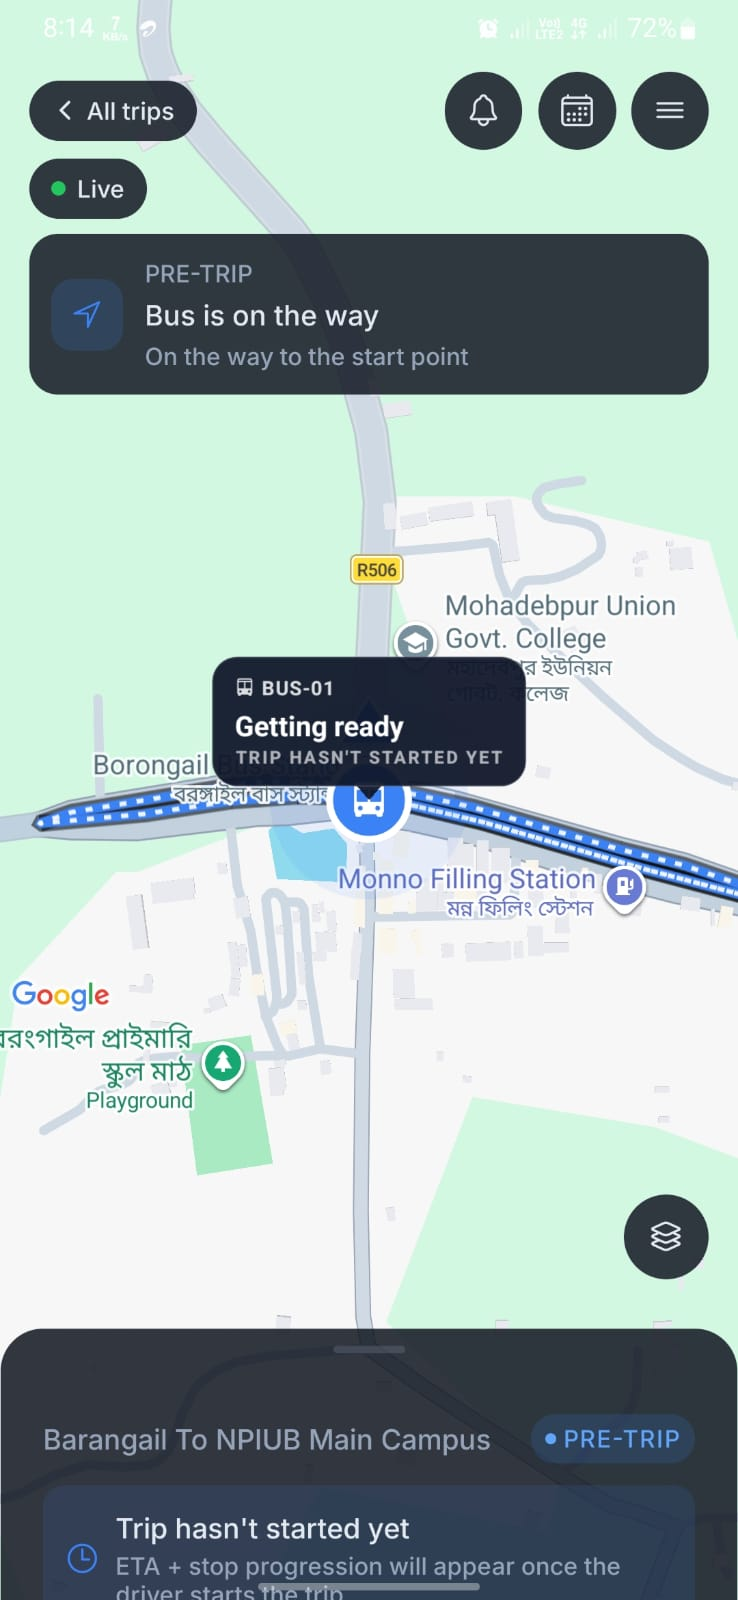
\includegraphics[width=0.235\textwidth]{shots/pretrip_map.jpg}\hfill
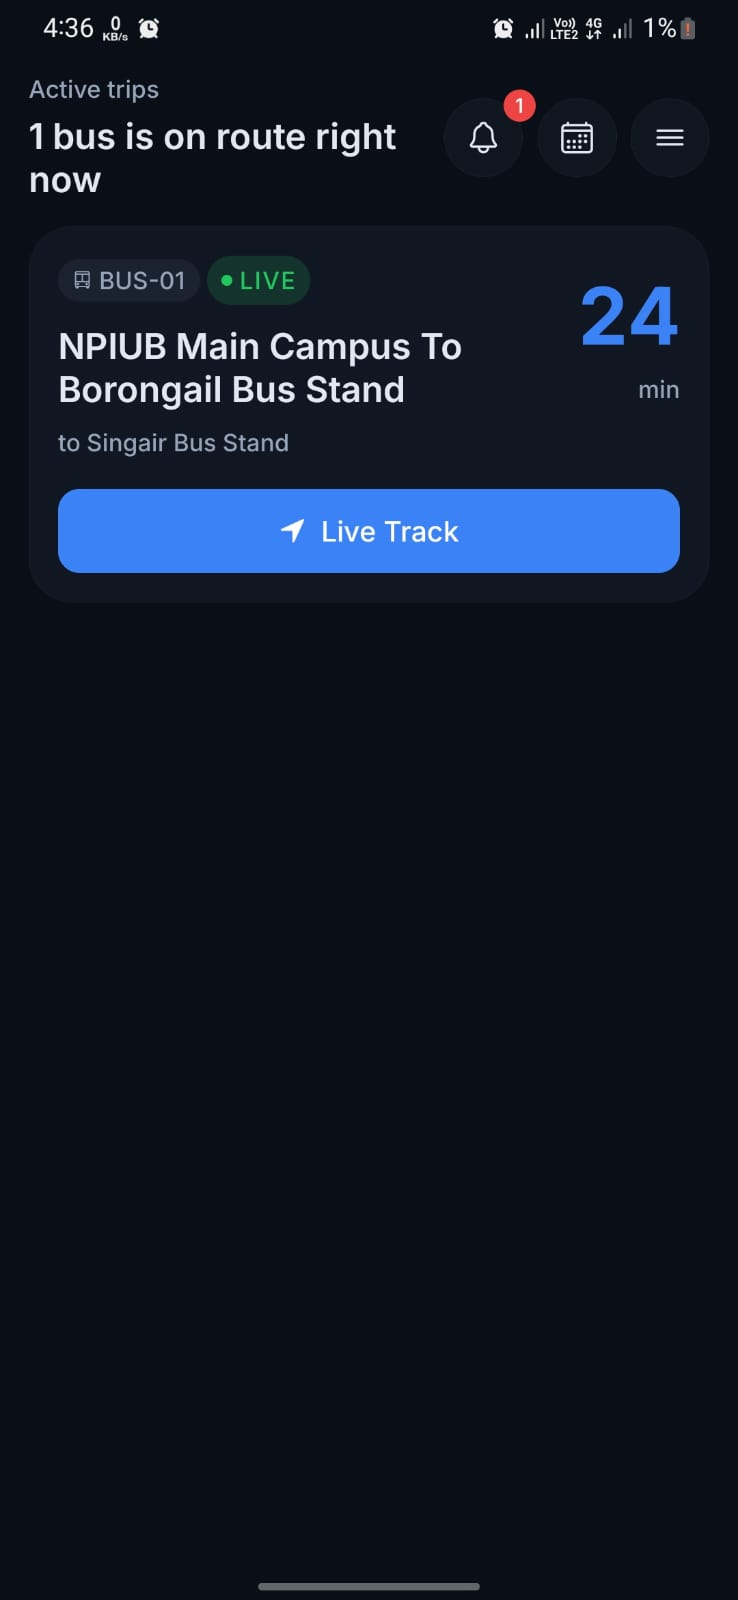
\includegraphics[width=0.235\textwidth]{shots/active_trip.jpg}\hfill

\includegraphics[width=0.235\textwidth]{shots/schedules.jpg}\hfill
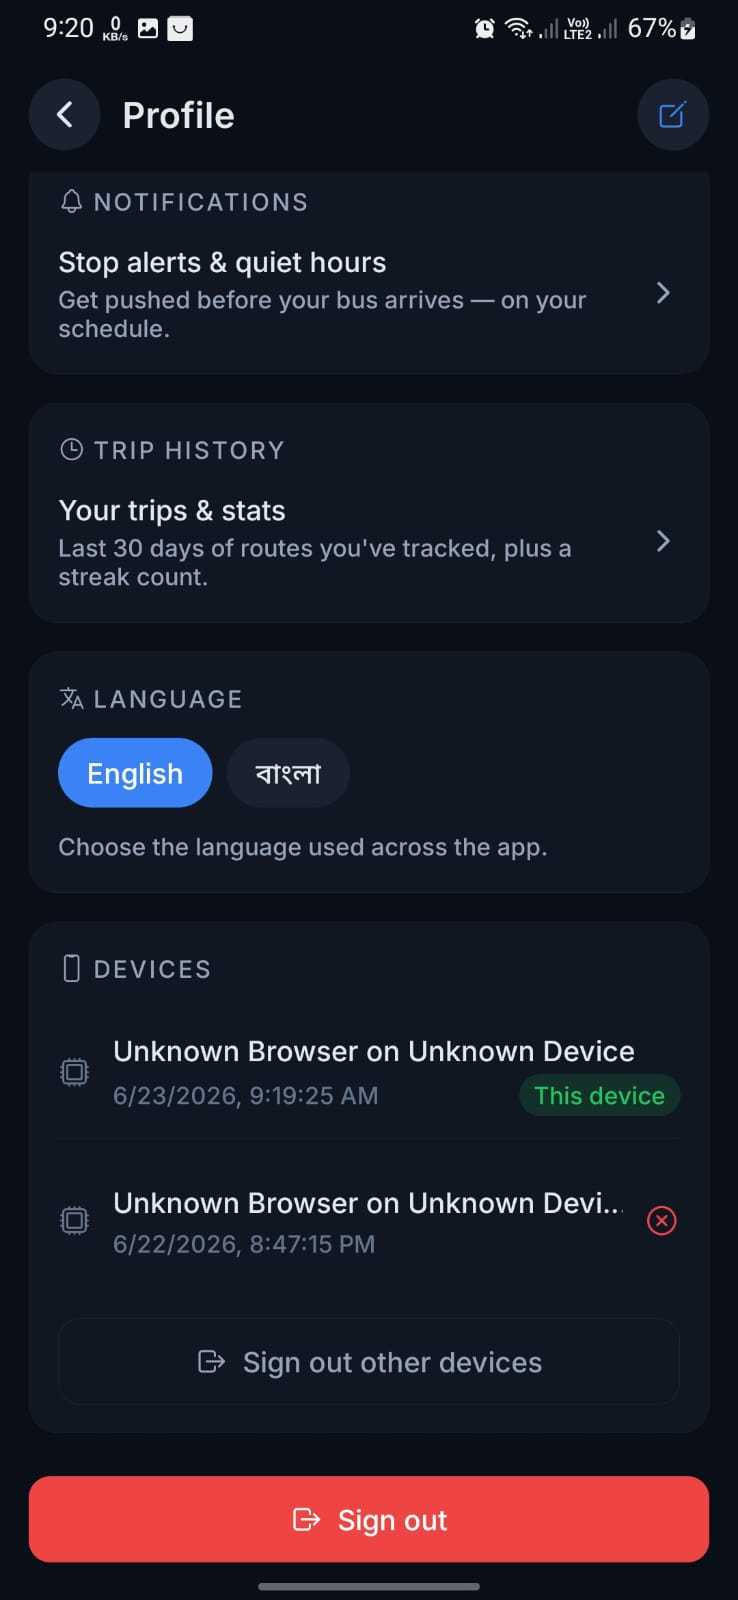
\includegraphics[width=0.235\textwidth]{shots/language.jpg}
\caption[Core tracking screens of the passenger application]{Core
tracking experience. Left to right: (a) the live map during the
\textsc{pre\_trip} window---the bus is rendered at its pre-departure
position with a ``getting ready'' state, so the map is never blank
before departure; (b) the active-trips view showing a live bus
(\textsc{bus-01}) on route with its ETA to the rider's stop and a
one-tap \emph{Live Track} action; (c) today's schedules grouped by day
and route; (d) the in-app language setting with the English/Bangla
toggle.}
\label{fig:screens-app}
\end{figure}

\begin{figure}[H]
\centering
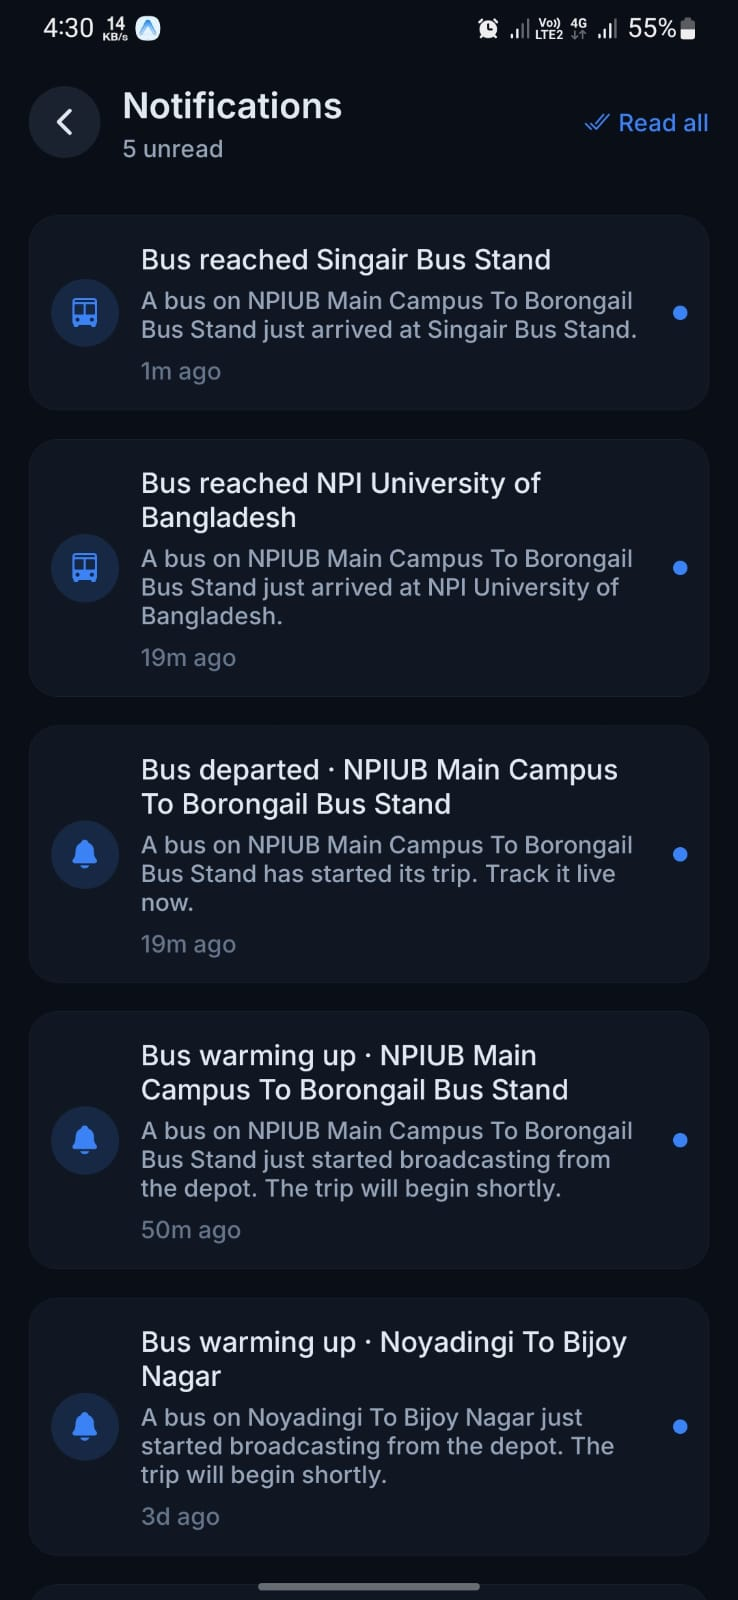
\includegraphics[width=0.235\textwidth]{shots/notif_list.jpg}\hfill
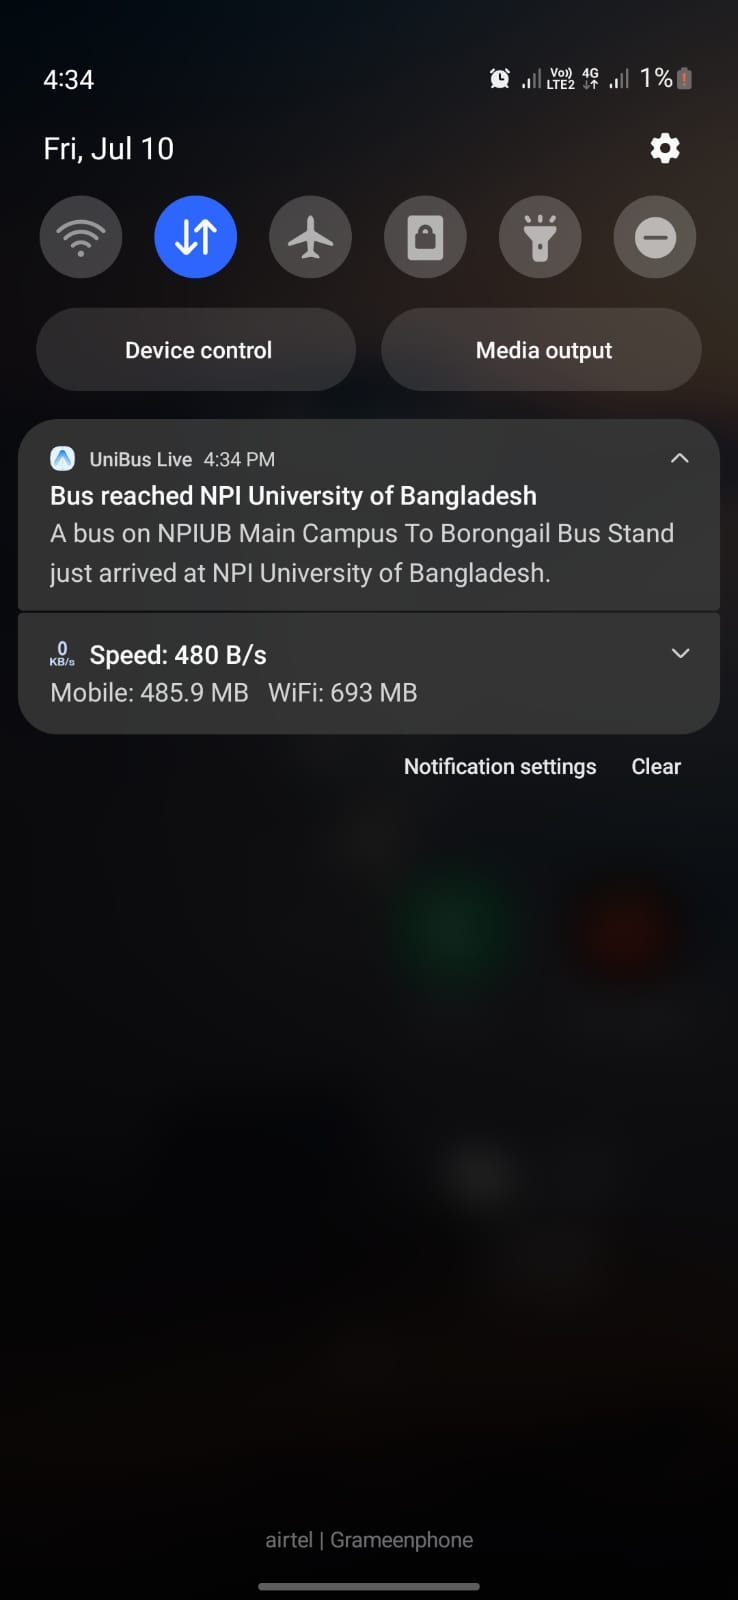
\includegraphics[width=0.235\textwidth]{shots/notif_shade.jpg}\hfill
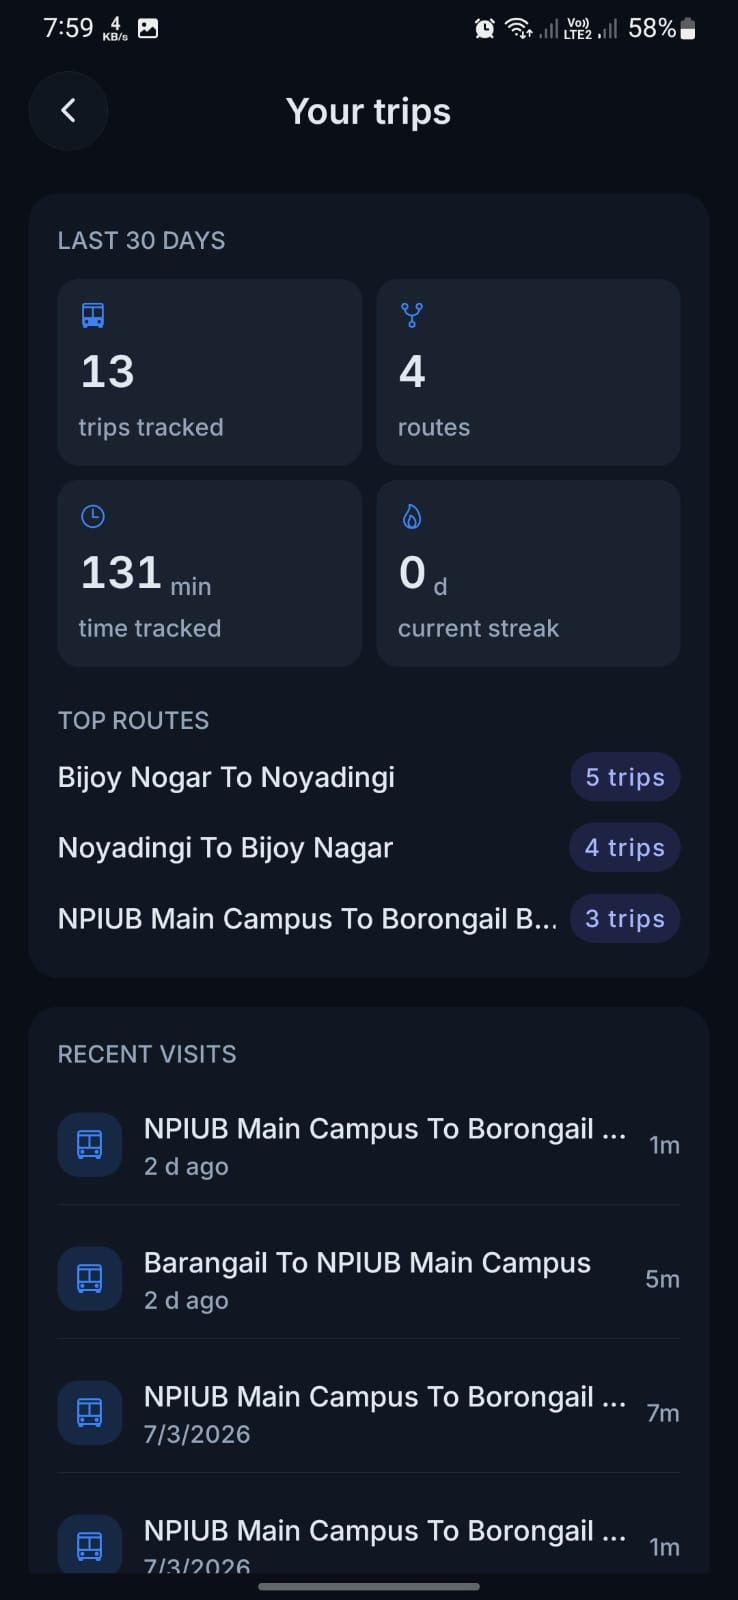
\includegraphics[width=0.235\textwidth]{shots/trip_stats.jpg}\hfill
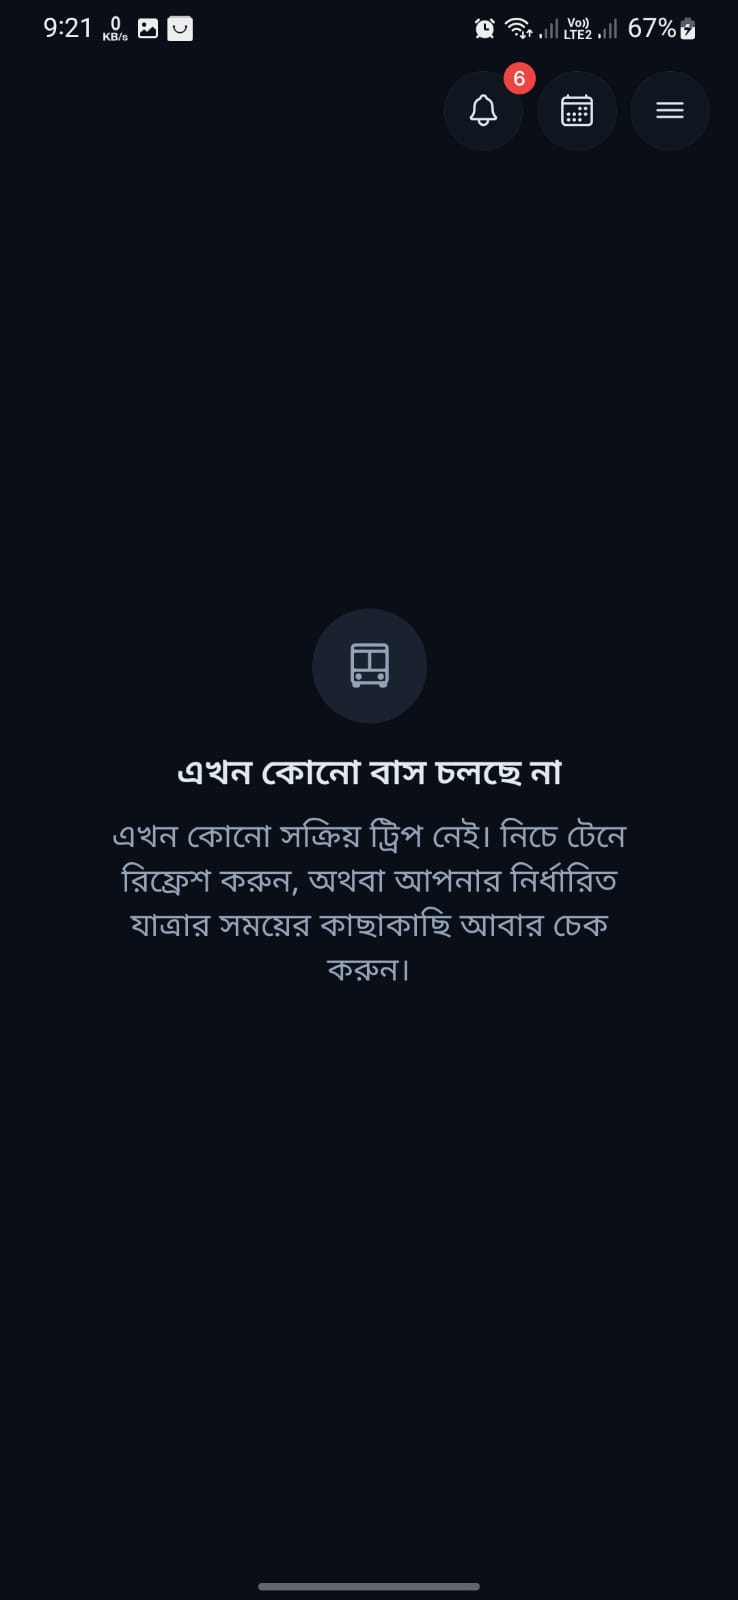
\includegraphics[width=0.235\textwidth]{shots/empty_bn.jpg}
\caption[Alerting and engagement screens]{Alerting and engagement
surfaces. Left to right: (a) the in-app notification feed recording trip
events (bus warming up, departed, reached a stop); (b) a system push
notification delivered outside the app announcing that the bus reached
the campus; (c) the rider's trip history and statistics (trips tracked,
routes used, time tracked); (d) the Bangla-localized empty state shown
when no bus is currently running---an example of the fully bilingual
interface (FR-10).}
\label{fig:screens-alerts}
\end{figure}

\chapter{Administration Console Screens}
\label{app:adminscreens}
This appendix reproduces the management pages of the web administration
console that complement the principal screens shown in
Figure~\ref{fig:admin}. All screens were captured from the deployed
console operating on the real fleet data.

\begin{figure}[H]
\centering
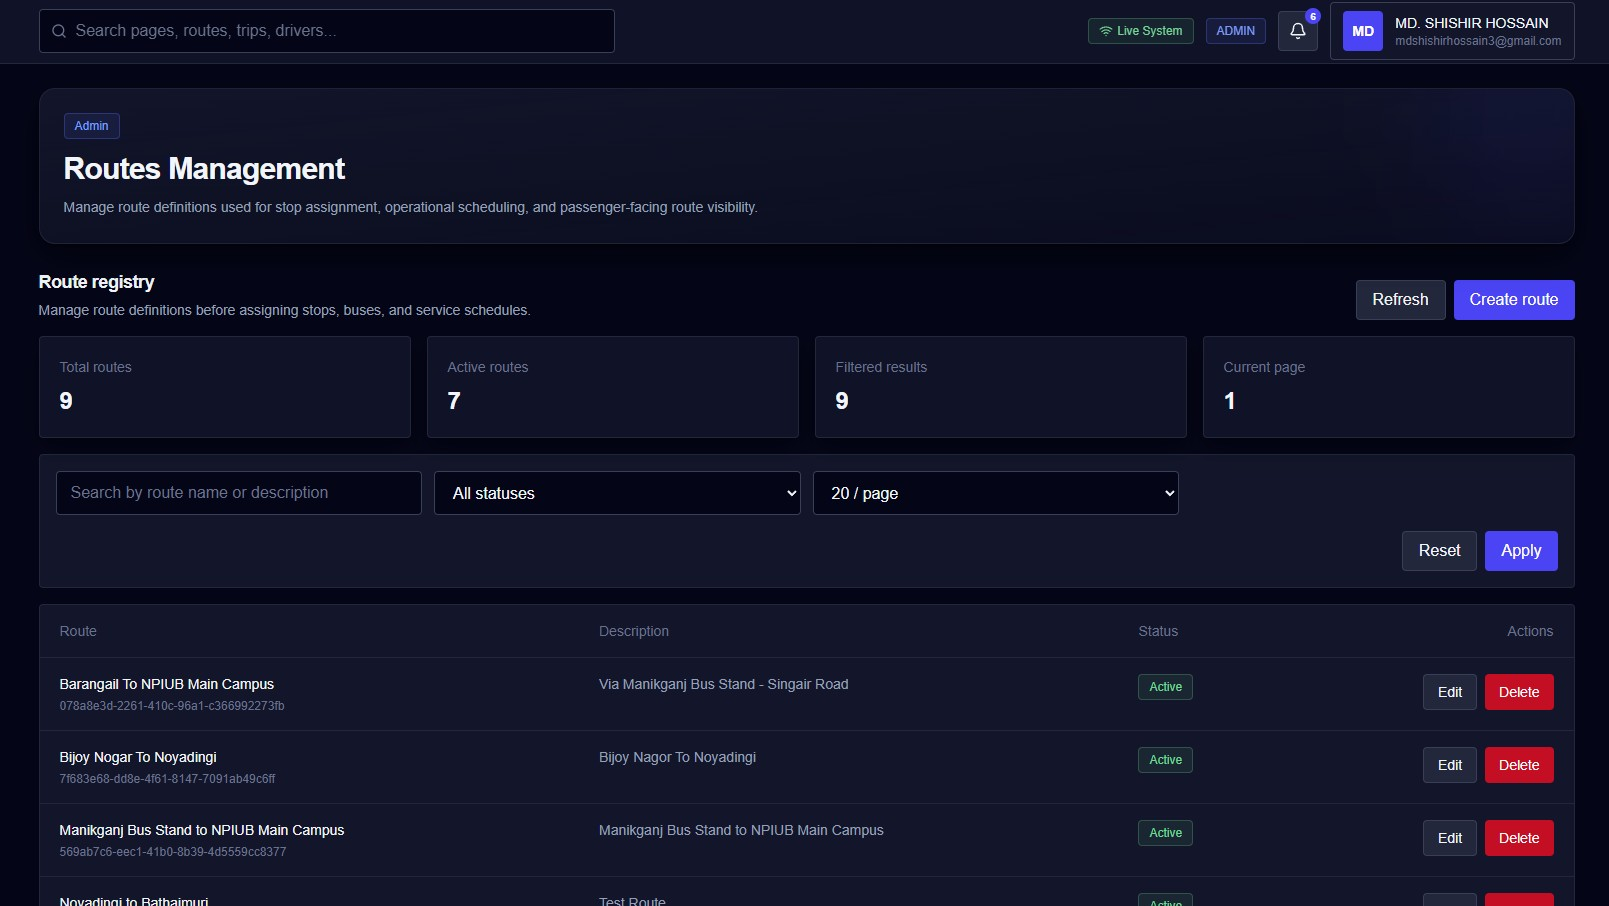
\includegraphics[width=0.49\textwidth]{admin/routes.jpg}\hfill
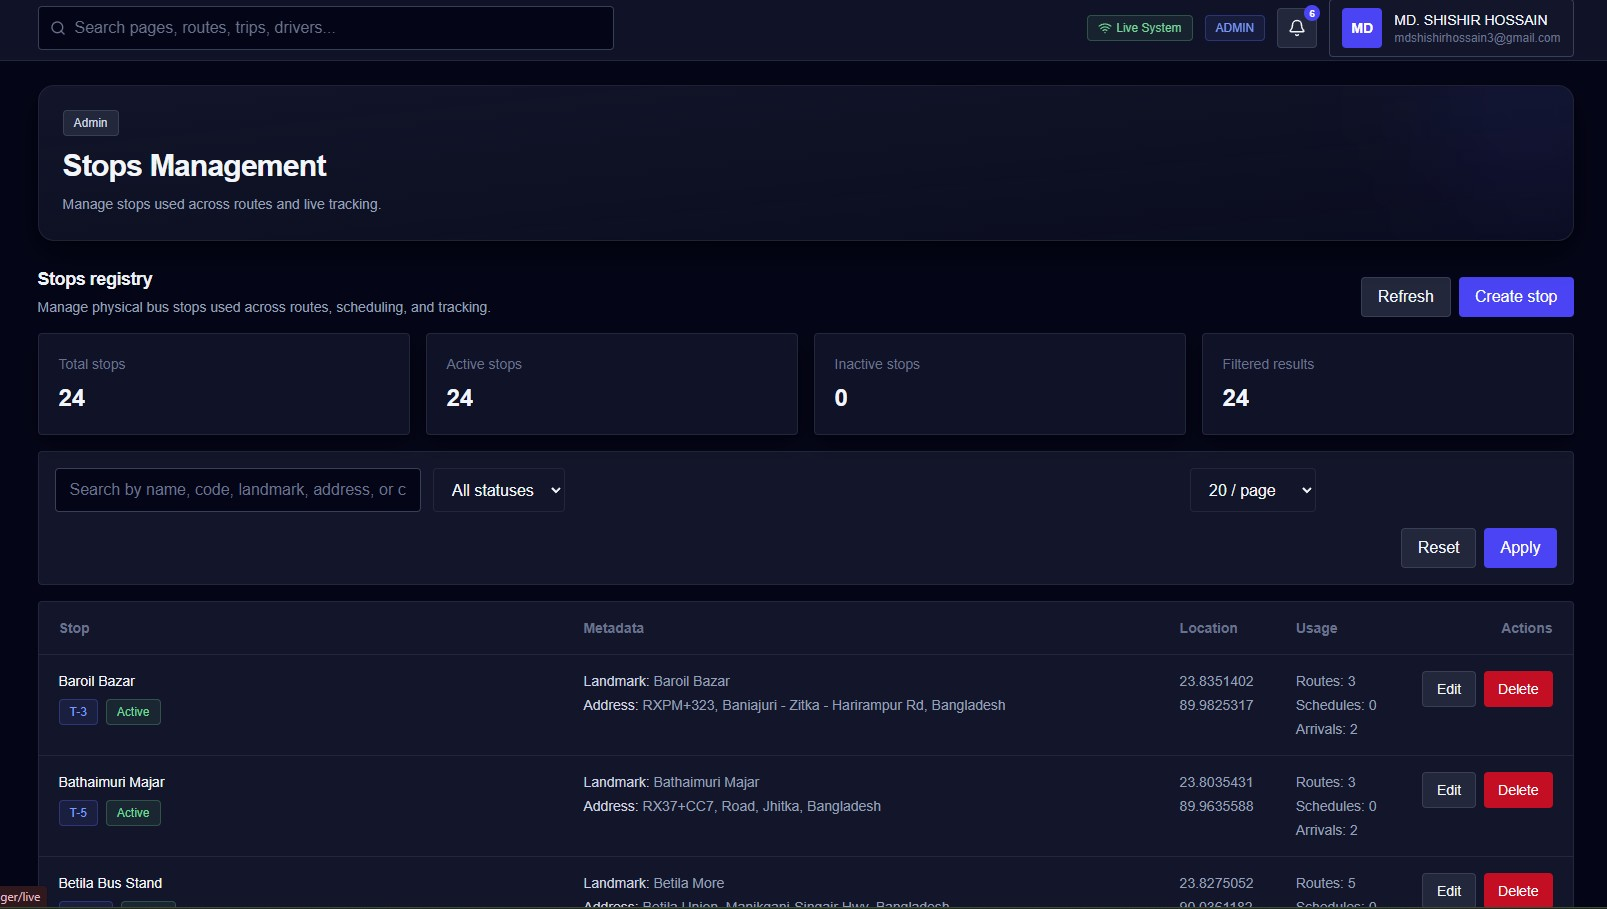
\includegraphics[width=0.49\textwidth]{admin/stops.jpg}\\[2mm]
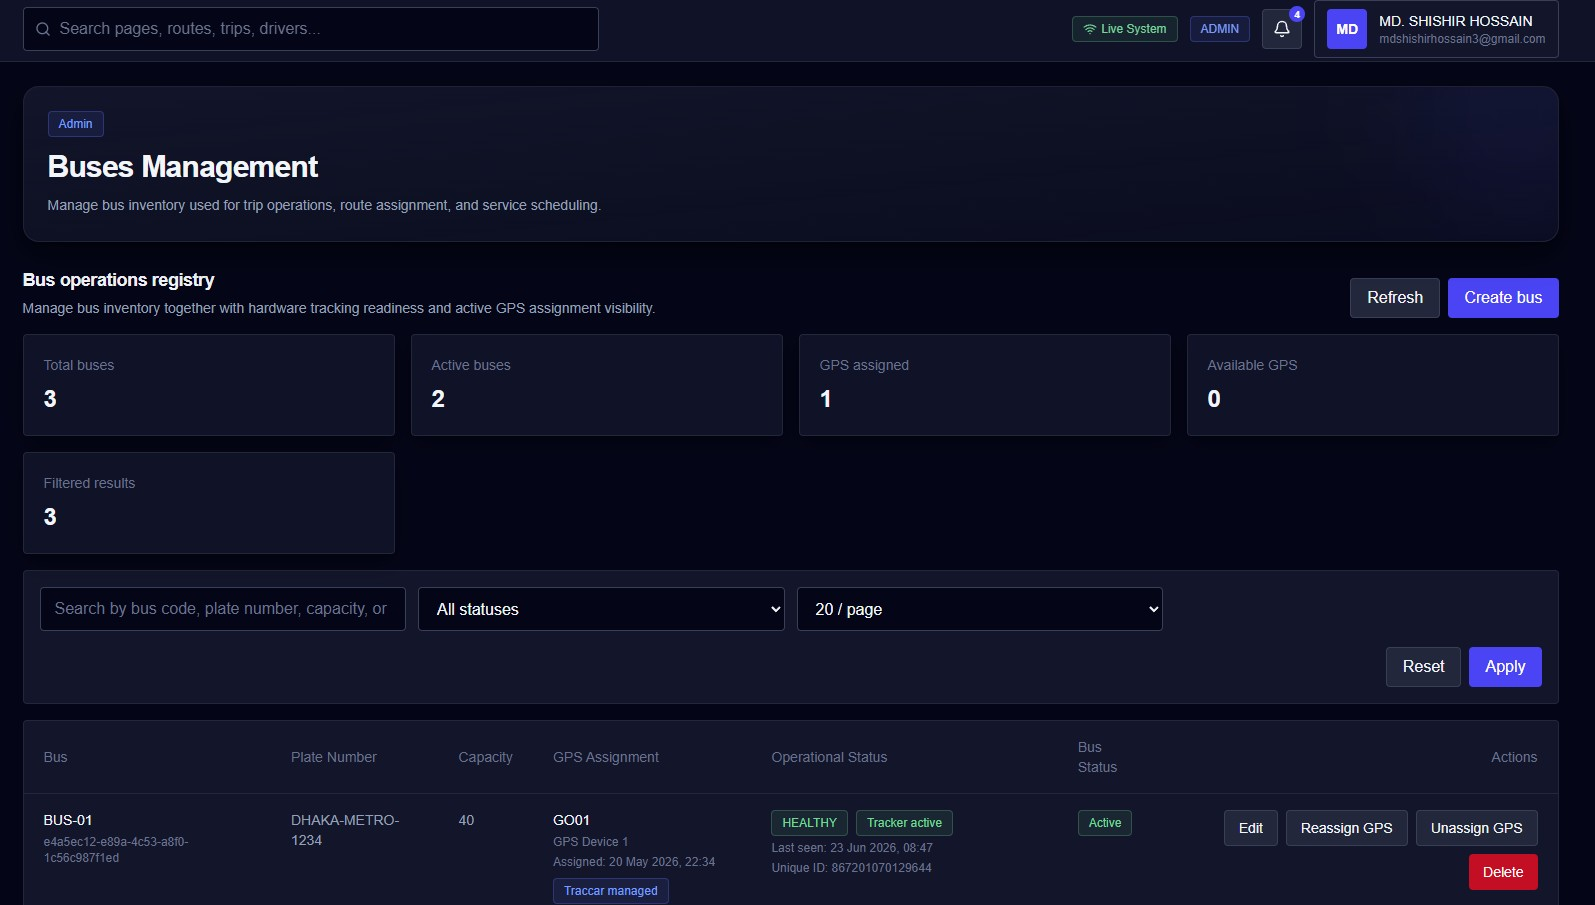
\includegraphics[width=0.49\textwidth]{admin/buses.jpg}\hfill
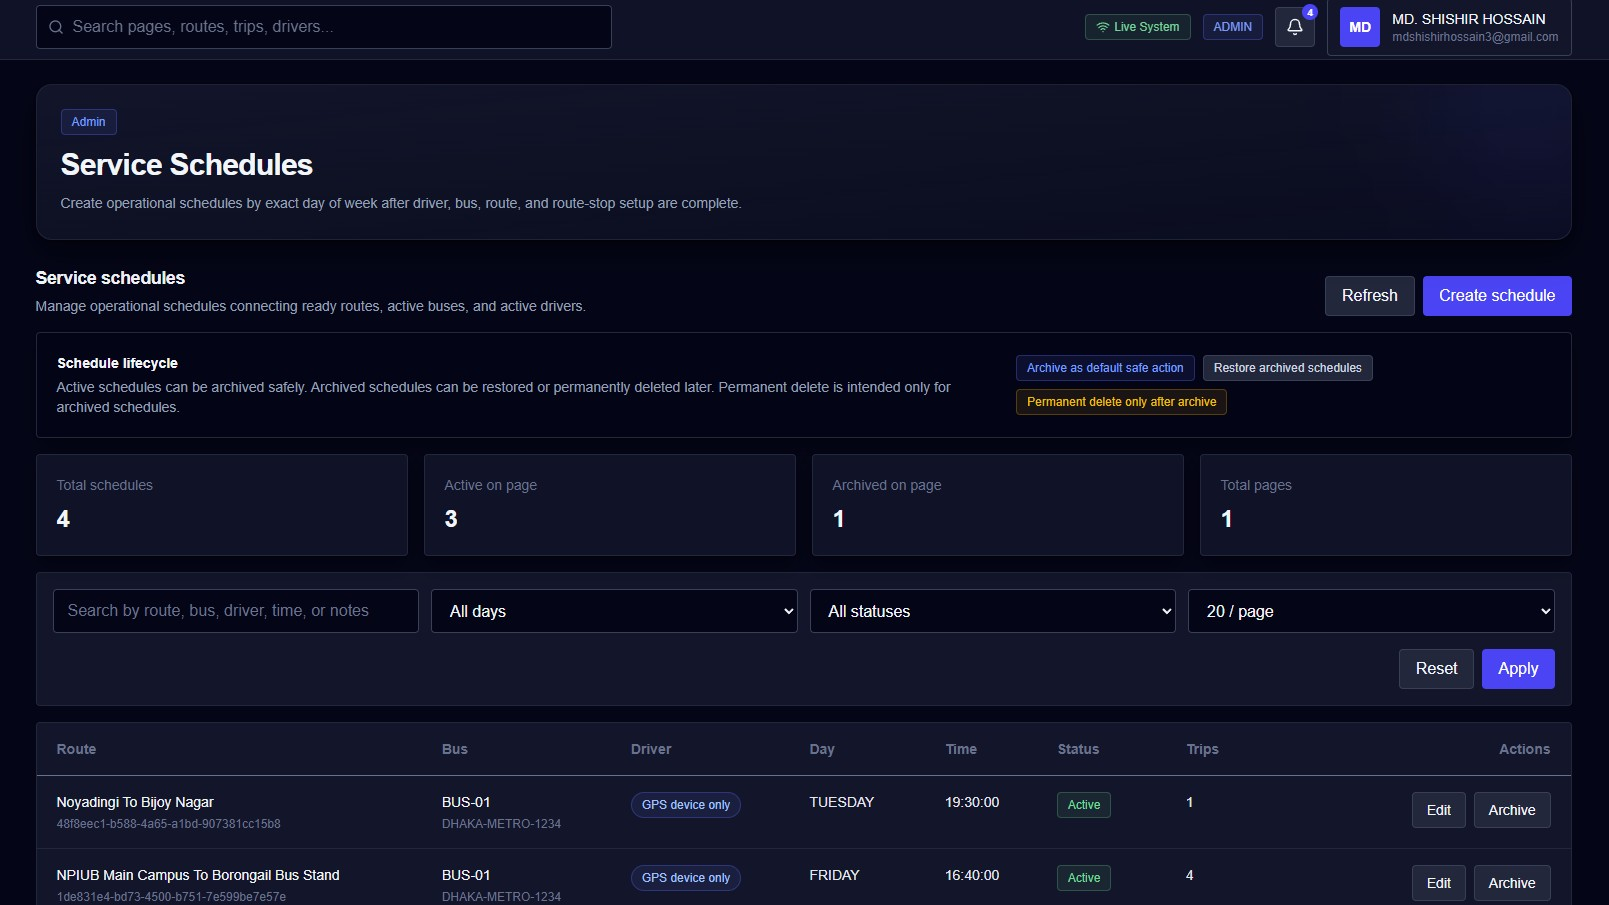
\includegraphics[width=0.49\textwidth]{admin/schedules.jpg}
\caption[Management pages of the administration console]{Management
pages of the administration console. Top left: the route registry with
per-route status and stop-visibility settings. Top right: stops
management, maintaining the physical bus stops used across routes.
Bottom left: bus operations registry, pairing each bus with its hardware
tracking readiness and GPS assignment. Bottom right: service schedules,
binding routes, buses, drivers, days, and departure times.}
\label{fig:admin-mgmt}
\end{figure}

\begin{figure}[H]
\centering
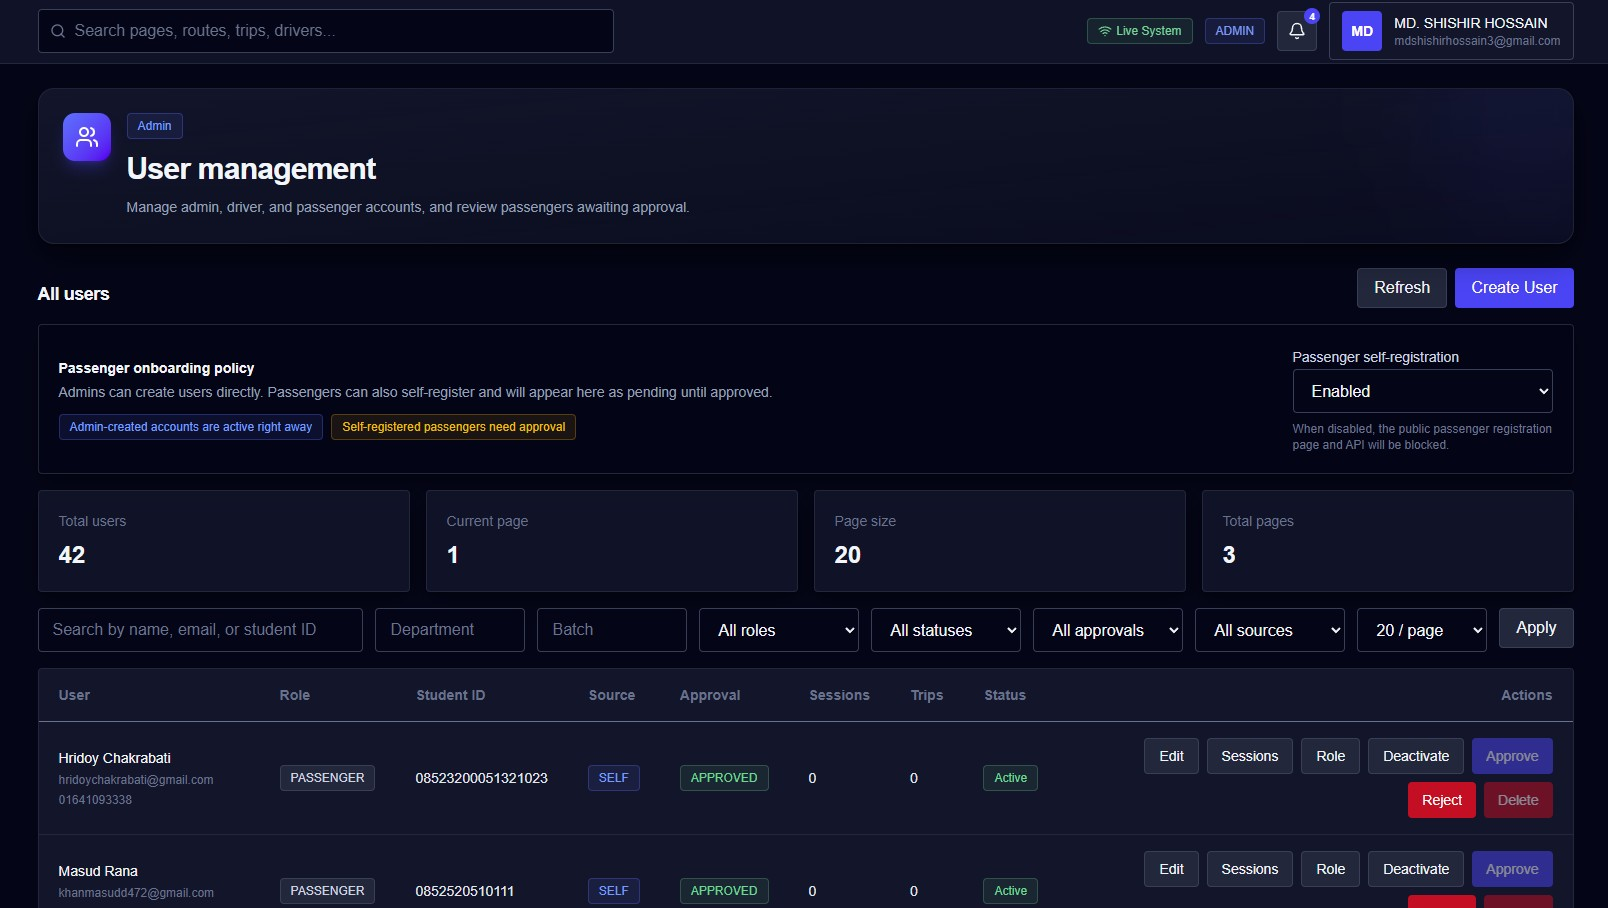
\includegraphics[width=0.85\textwidth]{admin/users.jpg}
\caption[User management page]{The user management page: accounts,
roles, per-user sessions, and the passenger onboarding approval policy
(NFR-5).}
\label{fig:admin-users}
\end{figure}


\end{document}
